%Version 3.1 December 2024
\documentclass[pdflatex, sn-nature]{sn-jnl}

%%%% Standard Packages
\usepackage{graphicx}%
\usepackage{multirow}%
\usepackage{amsmath,amssymb,amsfonts}%
\usepackage{amsthm}%
\usepackage{mathrsfs}%
\usepackage[title]{appendix}%
\usepackage{xcolor}%
\usepackage{textcomp}%
\usepackage{manyfoot}%
\usepackage{booktabs}%
\usepackage{algorithm}%
\usepackage{algorithmicx}%
\usepackage{algpseudocode}%
\usepackage{listings}%
\usepackage{siunitx}
\usepackage{cleveref}
%%%%

\graphicspath{{../Image/SI/}}

\crefname{figure}{Supplementary Figure}{Supplementary Figures}
\crefname{table}{Supplementary Table}{Supplementary Tables}
\crefname{section}{Supplementary Note}{Supplementary Notes}


\theoremstyle{thmstyleone}%
\newtheorem{theorem}{Theorem}%
\newtheorem{proposition}[theorem]{Proposition}% 

\theoremstyle{thmstyletwo}%
\newtheorem{example}{Example}%
\newtheorem{remark}{Remark}%

\theoremstyle{thmstylethree}%
\newtheorem{definition}{Definition}%

\setcounter{section}{0}
% \renewcommand{\thesection}{Supplementary Note \arabic{section}:}
\renewcommand{\thefigure}{S\arabic{figure}}
\renewcommand{\thetable}{S\arabic{table}}

\newcommand{\SupplementarySection}[1]{%
  \refstepcounter{section}%
  \section*{Supplementary Note \thesection: #1}%
  \addcontentsline{toc}{section}{Supplementary Note \thesection: #1}%
}

\raggedbottom


\begin{document}

\title[]{Supplementary Information for: Spatiotemporal Coherence of Cutaneous Shear Waves, Not Local Extrema, Dictates Mid-Air Tactile Perception}

\author[1]{\fnm{Linhan} \sur{Fan}}\email{linhanfan@seu.edu.cn}

\author[1]{\fnm{Zhutao} \sur{Wang}}\email{xxxx@seu.edu.cn}

\author[1]{\fnm{Hua} \sur{He}}\email{xxxx@seu.edu.cn}

\author*[1]{\fnm{Yafeng} \sur{Niu}}\email{nyf@seu.edu.cn}

\affil*[1]{\orgdiv{School of Mechanical Engineering}, \orgname{Southeast University}, \orgaddress{\city{Nanjing}, \country{China}}}

\maketitle



\SupplementarySection{Background of the ultrasound mid-air haptic}
\label{sec:background_ultrasound_mid_air_haptic}

Ultrasound mid-air haptics (UMH) technology delivers tactile feedback without physical contact by focusing airborne acoustic waves onto the skin surface~\cite{hoshiIntroductionUltrasonicMidair2022, rakkolainenSurveyMidAirUltrasound2021}. This interaction relies on acoustic radiation pressure, a non-linear effect arising from the momentum transfer of the acoustic field to an object~\cite{kingAcousticRadiationPressure1934a}. Because the acoustic impedance mismatch between air and human skin is approximately 99.9\%, incident ultrasound waves are almost entirely reflected. This reflection exerts a net force perpendicular to the skin surface~\cite{hoshiIntroductionUltrasonicMidair2022}. To produce perceptible forces, UMH systems employ phased arrays of transducers to generate constructive interference at specific spatial locations, creating a high-intensity acoustic focus~\cite{rakkolainenSurveyMidAirUltrasound2021, priceFibonacciSpiralArranged2018}.

Because the carrier frequency of these systems (typically \qty{40}{\kHz}) far exceeds the temporal sensitivity of cutaneous mechanoreceptors ($<\qty{1}{\kHz}$)~\cite{johnsonRolesFunctionsCutaneous2001, mountcastleNeuralBasisSense1967}, the acoustic field requires modulation to elicit tactile sensations. Amplitude Modulation (AM) varies the focal intensity at a perceptible frequency (e.g., \qty{200}{\Hz}) to activate Pacinian corpuscles~\cite{hoshiIntroductionUltrasonicMidair2022}. Alternatively, Spatiotemporal Modulation (STM) or Lateral Modulation (LM) rapidly steers the focal point along a trajectory on the skin~\cite{takahashiTactileStimulationRepetitive2020}. This scanning approach distributes acoustic energy over a larger area and generates shear shock waves in the skin, which enhances the perceived intensity and spatial extent of the tactile stimuli~\cite{reardonCutaneousWavePropagation2019, reardonShearShockWaves2023}.





\SupplementarySection{Ultrasound mid-air haptic device details}
\label{sec:umh_device_details}


\begin{figure}[htbp]
    \centering
    \includegraphics[width=\textwidth]{Figure_UMH_Device.pdf}
    \caption{\textbf{Overview of the custom-built Ultrasound Mid-Air Haptic (UMH) device.} \textbf{a}, Isometric view of the assembled device showing the compact hexagonal form factor. \textbf{b}, Top view of the acoustic aperture consisting of 60 ultrasonic transducers arranged in a hexagonal close-packed lattice with a central cutout for a CMOS sensor. \textbf{c}, Bottom view of the main control PCB, housing the STM32H750 microcontroller, USB-C data interface, and power management circuits. \textbf{d}, Side profile showing the USB-C data and debugging interfaces. \textbf{e}, Side profile showing the 12V DC power input jack. \textbf{f}, Bottom view of the transducer driver board. \textbf{g}, Detailed view of the driver circuitry for individual channels, highlighting the IX4428MTR driver ICs, TVS protection diodes, and status LEDs.}
    \label{fig:supplementary_figure_umh_device}
\end{figure}

\begin{figure}[htbp]
    \centering
    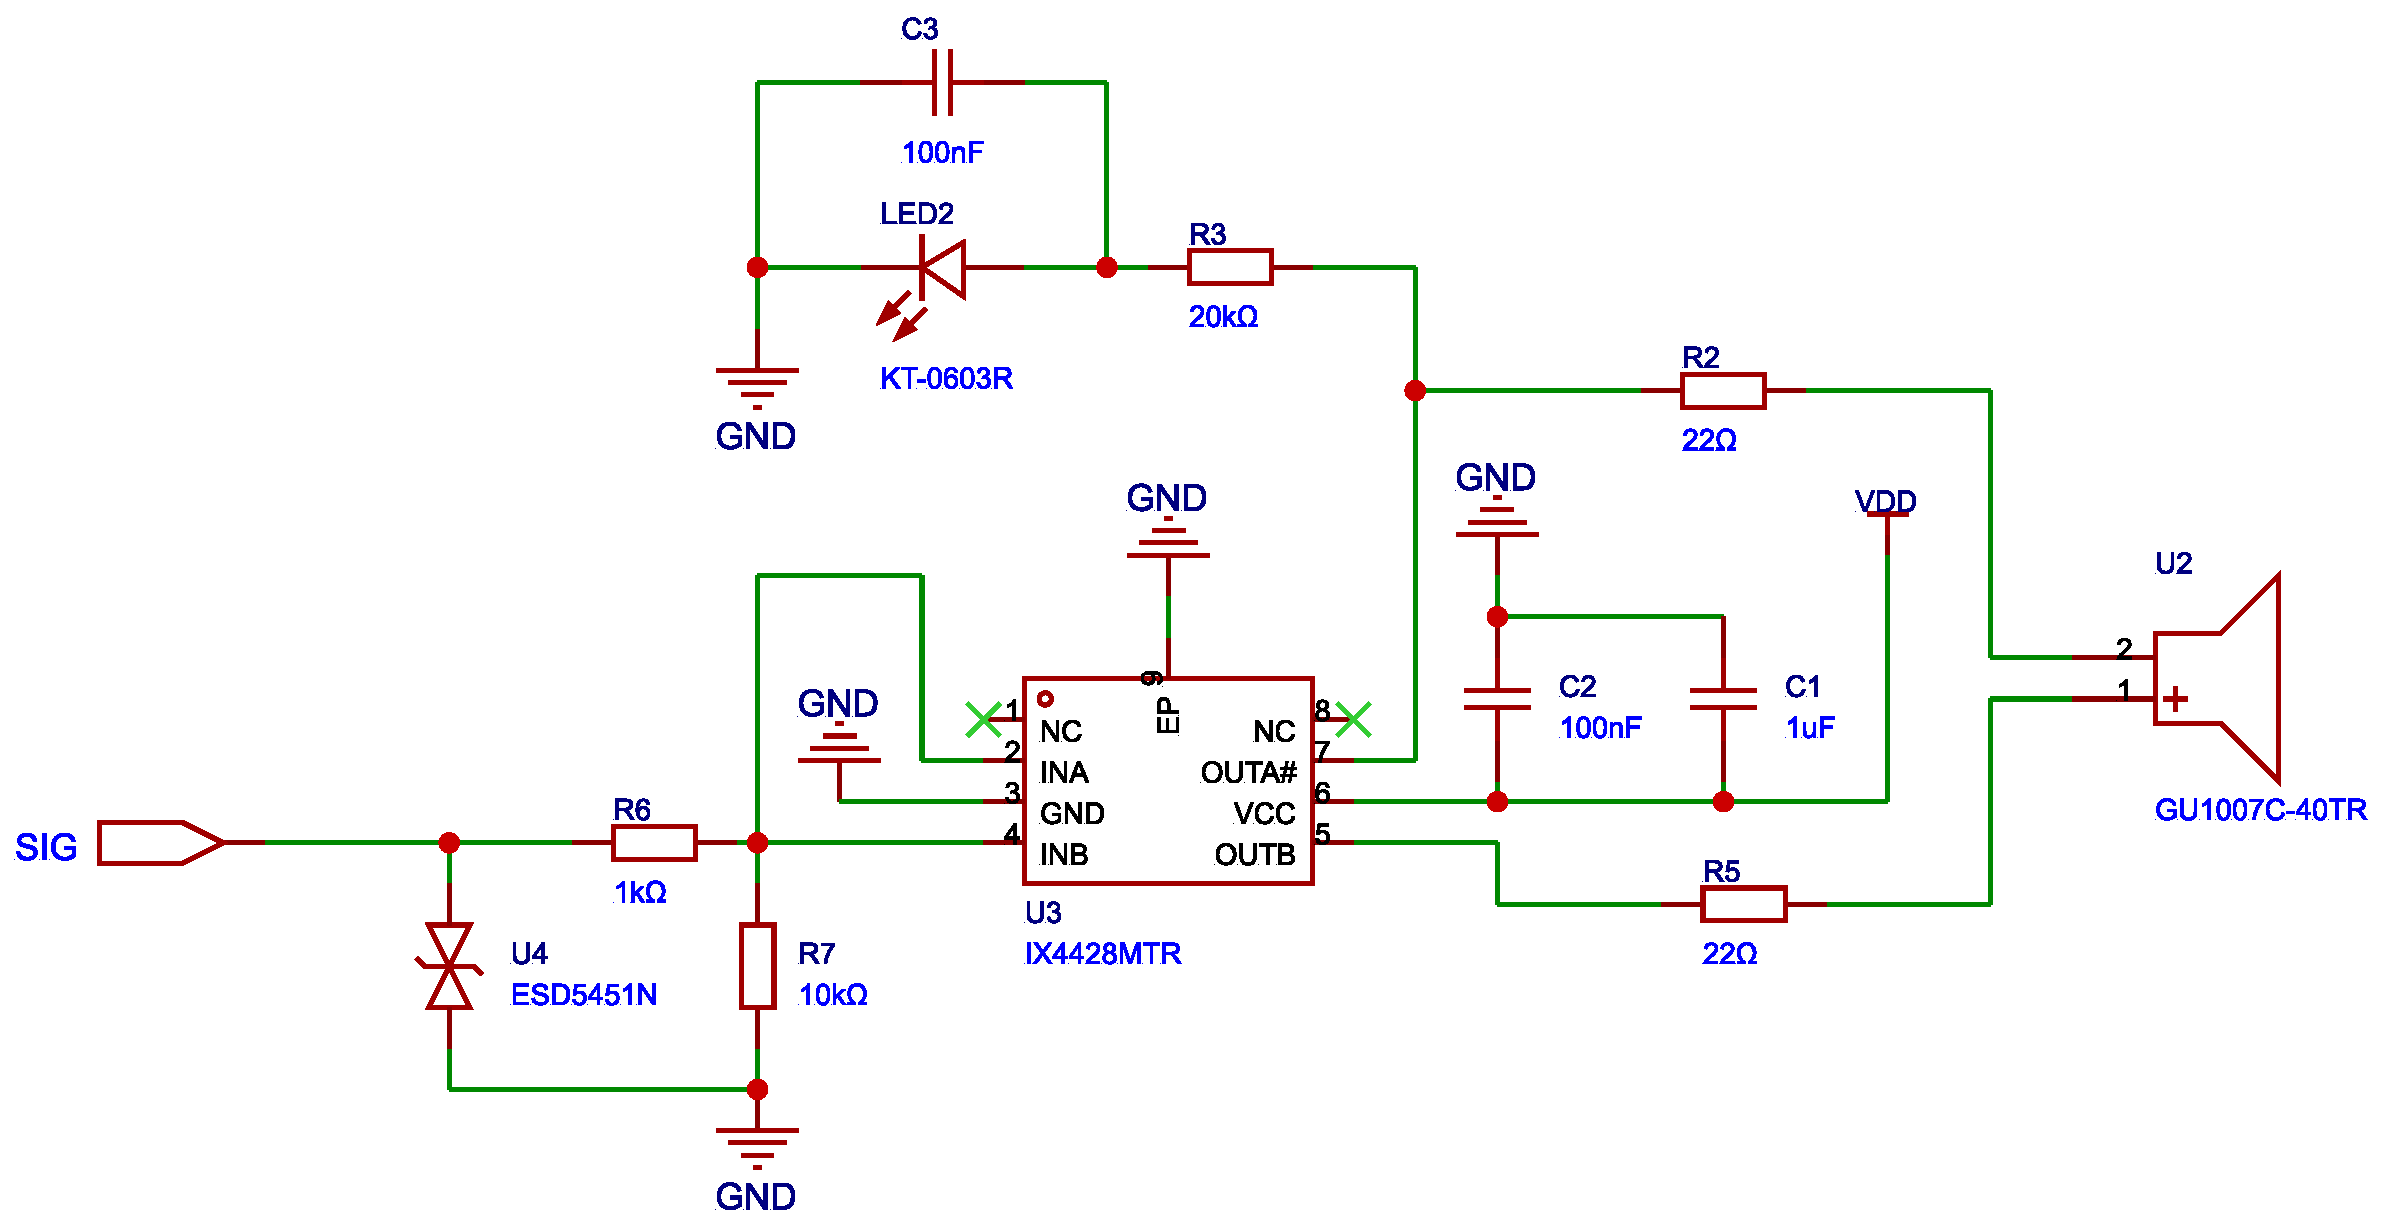
\includegraphics[width=\textwidth]{Figure_Transducer_Driver_Circuit.pdf}
    \caption{\textbf{Schematic of the single-channel ultrasonic transducer driver circuit.} The digital control signal (SIG) is buffered and inverted by the IX4428MTR driver IC to generate complementary outputs (OUTA and OUTB). This bipolar drive topology applies a \qty{24}{\volt} peak-to-peak square wave across the piezoelectric transducer (GU1007C-40TR) from a single \qty{12}{\volt} supply, maximizing acoustic emission. The circuit includes ESD protection and a visual status indicator.}
    \label{fig:supplementary_figure_transducer_driver_circuit}
\end{figure}


We developed a custom high-energy-density Ultrasound Mid-Air Haptic (UMH) device for this study (\cref{fig:supplementary_figure_umh_device}a). The system integrates a phased array of ultrasonic transducers, multi-channel driving circuitry, and a central processing unit into a compact hexagonal prism form factor (\qtyproduct{102.2 x 90 x 32.2}{\milli\meter}).


The acoustic aperture consists of 60 airborne ultrasonic transducers (GU1007C-40TR, Dongguan Ninghai Electronics Co., Ltd.) arranged in a hexagonal close-packed (HCP) lattice. The transducers have a diameter of \qty{10}{\milli\meter} and are spaced with a center-to-center pitch of \qty{10}{\milli\meter}, which maximizes the fill factor for efficient acoustic power generation. A central aperture accommodates a CMOS image sensor for future visual tracking integration (\cref{fig:supplementary_figure_umh_device}b). Each transducer operates at a center frequency of \qty{40}{\kilo\hertz} with a directivity of approximately \ang{80}.

A \qty{12}{\volt} DC input powers the device, regulated to provide \qty{3.3}{\volt} and \qty{5.0}{\volt} rails for logic and analog subsystems. The core control unit is an STM32H750VBT6 microcontroller (STMicroelectronics) based on the ARM Cortex-M7 core. The MCU handles communication with the host PC via a USB Type-C interface using the CDC virtual serial port protocol.

A Direct Memory Access (DMA) based signal generation mechanism controls the beamforming phase. The MCU's timer triggers DMA transfers at a sampling frequency of \qty{4}{\mega\hertz}, updating the output state of the GPIO ports. For the \qty{40}{\kilo\hertz} carrier wave, the system discretizes each acoustic cycle into 100 time slices, providing a phase resolution of $2\pi/100$ (temporal resolution of \qty{250}{\nano\second}).

The amplification stage uses a bipolar drive topology to maximize the acoustic pressure output from the available \qty{12}{\volt} supply. As illustrated in the schematic (\cref{fig:supplementary_figure_transducer_driver_circuit}), the logic-level signal (SIG) feeds into a dual-channel low-side MOSFET driver (IX4428MTR, IXYS Integrated Circuits Division). The driver outputs two complementary square waves (OUTA and OUTB) to the transducer terminals. This push-pull configuration doubles the voltage swing across the piezoelectric element to \qty{24}{\volt} peak-to-peak (Vpp). Each channel includes a transient voltage suppressor (TVS) diode (ESD5451N) for electrostatic discharge protection and a status LED for visual monitoring of channel activity (\cref{fig:supplementary_figure_umh_device}g).

\begin{figure}[htbp]
    \centering
    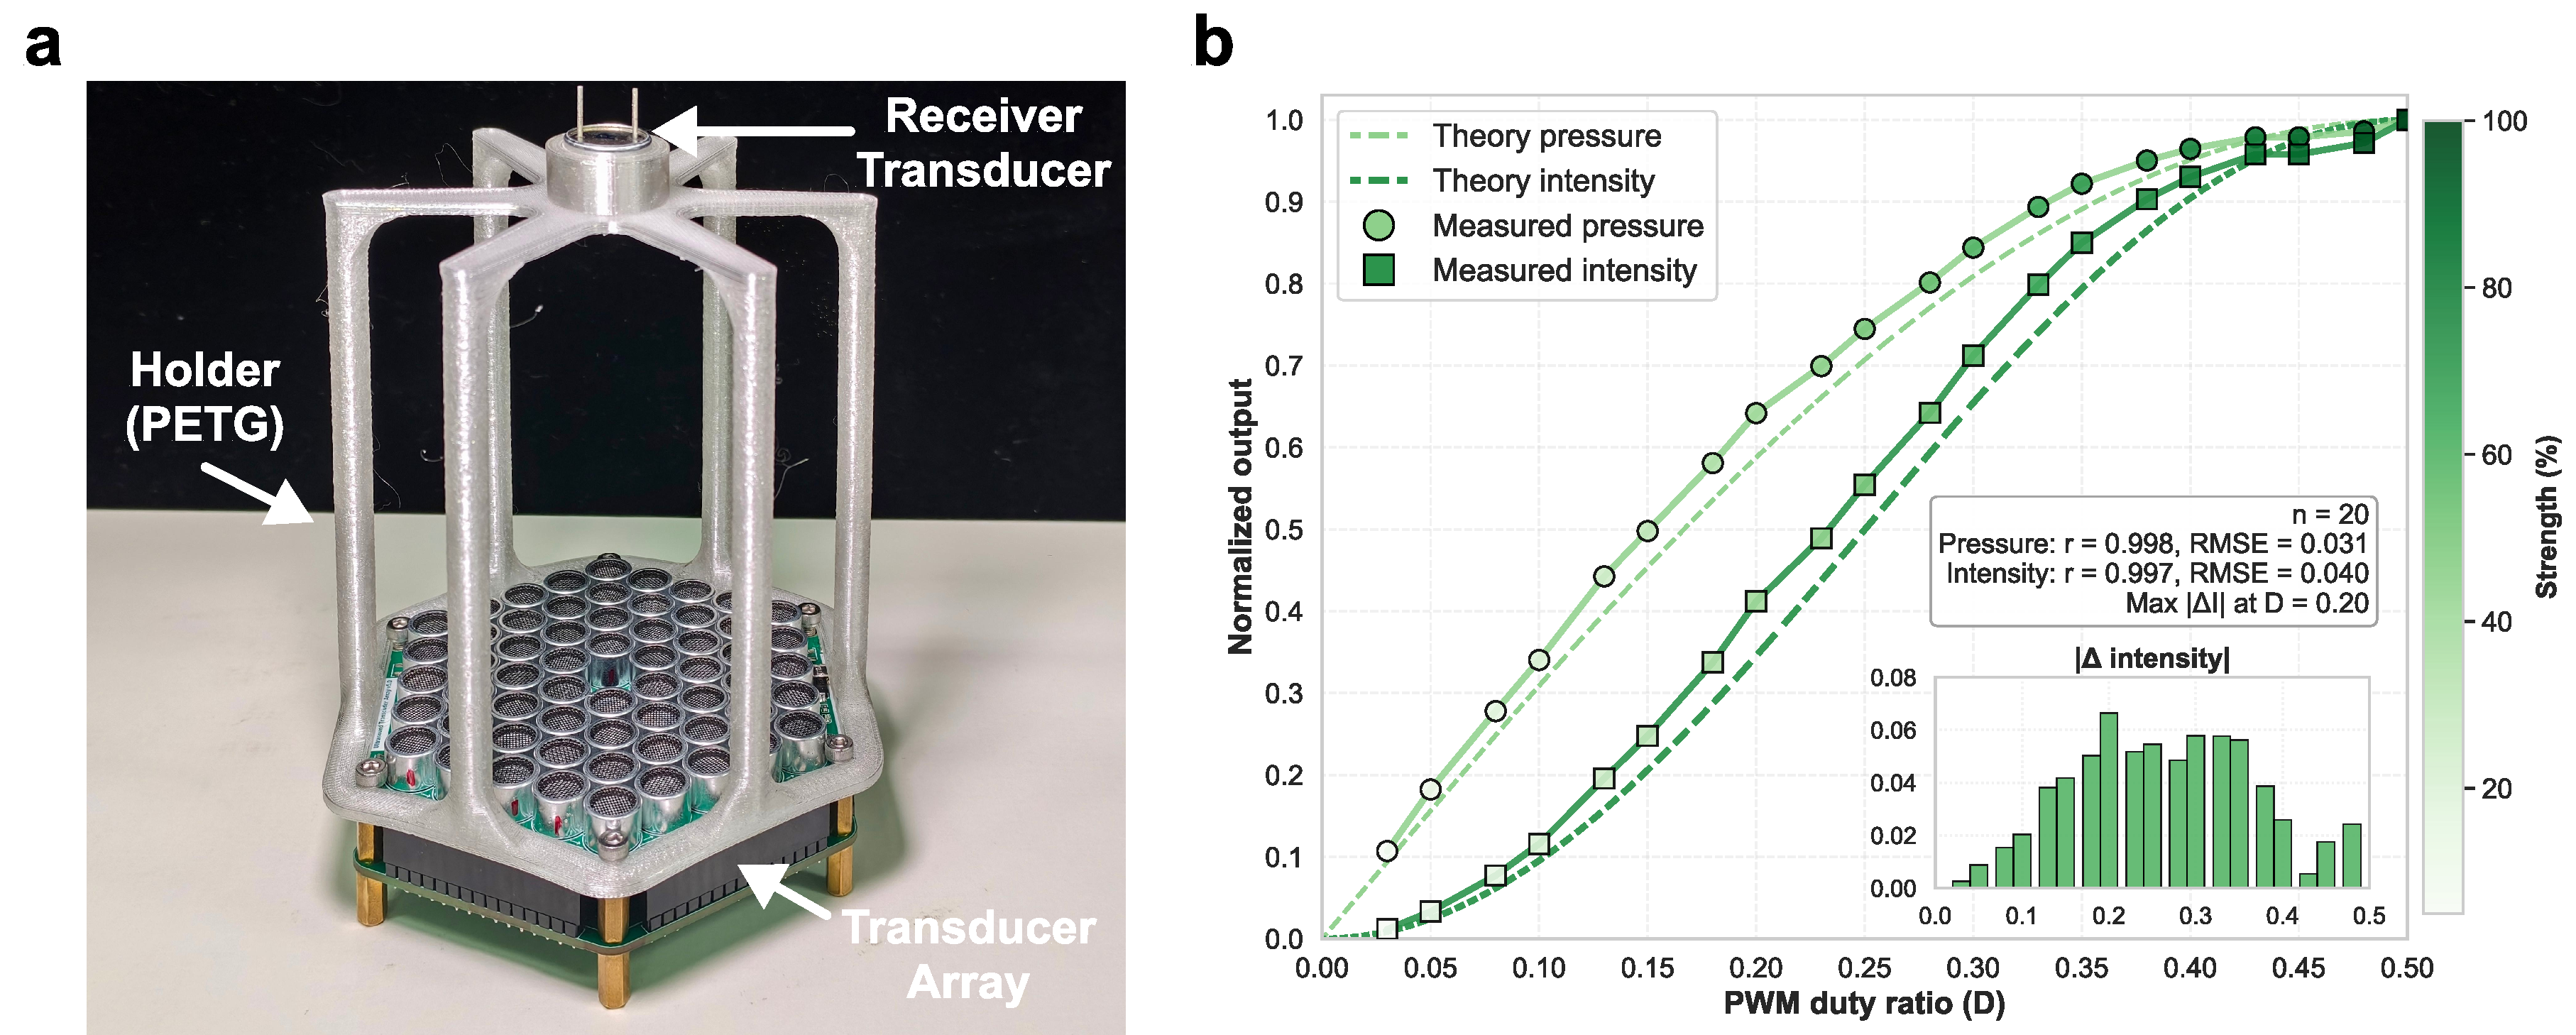
\includegraphics[width=\textwidth]{Figure_Intensity_Test.pdf}
    \caption{\textbf{Hardware calibration of the UMH device output magnitude and validation of the PWM-to-acoustic transfer function.} \textbf{a}, Photograph of the rigid calibration fixture used for acoustic output measurement. A receiver transducer identical to the emitting elements was mounted at the geometric focal position above the array by a custom 3D-printed PETG holder, thereby fixing the receiver at \qty{100}{\milli\meter} above the array center. \textbf{b}, Comparison between the theoretical transfer functions and the experimentally measured normalized output. The horizontal axis reports the PWM duty ratio $D$, which is linearly mapped from the firmware strength command. Light and dark green dashed curves indicate the theoretical normalized pressure and intensity, respectively. Circular markers show the measured normalized pressure, obtained from the received steady-state $V_{pp}$, and square markers show the corresponding normalized intensity inferred from the squared normalized voltage. The inset histogram summarizes the absolute intensity deviation $|\Delta I|$ between measurement and theory across all sampled duty ratios.}
    \label{fig:supplementary_figure_intensity_test}
\end{figure}

Experiment 2 required the device output to be adjustable in physically meaningful and approximately equal perceptual increments to support absolute detection-threshold measurements. However, the firmware controls ultrasonic emission strength through pulse-width modulation of the bipolar driver stage rather than through a linear acoustic amplitude source. As a result, the user-level strength parameter is not linearly proportional to the emitted acoustic pressure or to the resulting acoustic radiation force on the skin. Because the adaptive staircase procedure assumes a monotonic and well-characterized mapping between command level and physical stimulus magnitude, we derived and validated the transfer function from the PWM command to the effective acoustic output.

The derivation starts from the bipolar square-wave excitation applied to each transducer at the carrier frequency of \qty{40}{\kilo\hertz}. Let $D$ denote the one-sided PWM duty ratio within the available half-cycle control range, with $D \in [0,0.5]$. In the firmware, the dimensionless strength command $S \in [0,100]$ maps linearly to the duty ratio according to
\begin{equation}
    D = 0.5\frac{S}{100}.
\end{equation}
For a bipolar rectangular waveform with duty ratio $D$, Fourier decomposition shows that the amplitude of the fundamental \qty{40}{\kilo\hertz} component is proportional to $\sin(\pi D)$. Since focal acoustic pressure is proportional to the carrier-frequency fundamental voltage component, the normalized acoustic pressure is
\begin{equation}
    P_{\mathrm{norm}}(D) = \sin(\pi D).
\end{equation}
Substituting the strength mapping yields the equivalent command-domain expression
\begin{equation}
    P_{\mathrm{norm}}(S) = \sin\!\left(\frac{\pi}{2}\frac{S}{100}\right).
\end{equation}
Under the standard approximation that acoustic intensity and radiation-force magnitude scale with squared acoustic pressure, the corresponding normalized intensity transfer function becomes
\begin{equation}
    I_{\mathrm{norm}}(D) = P_{\mathrm{norm}}^2(D) = \sin^2(\pi D),
\end{equation}
or equivalently
\begin{equation}
    I_{\mathrm{norm}}(S) = \sin^2\!\left(\frac{\pi}{2}\frac{S}{100}\right).
\end{equation}
These expressions define the ideal command-to-output transfer law expected from the hardware if the transducer, driver, and acoustic propagation stages remain approximately linear at the carrier frequency.

We performed a benchtop calibration experiment to test this prediction. The measurement setup is shown in \cref{fig:supplementary_figure_intensity_test}a. A custom 3D-printed PETG holder mechanically registered to the outer geometry of the phased-array housing. The holder positioned a receiver transducer of the same model as the transmitting elements directly above the geometric center of the array at the nominal focus location $(0,0,\qty{0.1}{\meter})$. This arrangement minimized placement variability and ensured that all recordings occurred at a fixed spatial point coincident with the focal target used in the psychophysical experiments.

During calibration, we configured the UMH device in a static single-focus mode, keeping the focal point fixed at the center of the measurement volume. We swept the strength command from $S=5$ to $S=100$ in increments of 5, corresponding to 20 sampled duty ratios from $D=0.025$ to $D=0.5$. At each setting, we recorded the steady-state peak-to-peak voltage $V_{pp}(S)$ generated across the receiver transducer terminals using an oscilloscope (DS1104, RIGOL TECHNOLOGIES CO., LTD). The maximum measured value occurred at full-scale drive, where $V_{pp}(100)=\qty{14.1}{\volt}$. We then formed the measured normalized pressure as
\begin{equation}
    \widehat{P}_{\mathrm{norm}}(S)=\frac{V_{pp}(S)}{V_{pp}(100)},
\end{equation}
and the measured normalized intensity as
\begin{equation}
    \widehat{I}_{\mathrm{norm}}(S)=\left[\frac{V_{pp}(S)}{V_{pp}(100)}\right]^2.
\end{equation}
This normalization removes the absolute gain factor of the receiver chain and allows a direct comparison between theory and experiment at the level of transfer-function shape.

The measured data closely followed the theoretical sinusoidal transfer law over the full command range (\cref{fig:supplementary_figure_intensity_test}b). For normalized pressure, the correlation between measurement and theory was $r=0.998$ with a root-mean-square error of $\mathrm{RMSE}=0.031$. For normalized intensity, the agreement remained similarly high, with $r=0.997$ and $\mathrm{RMSE}=0.040$. These values indicate that the hardware reproduces the expected nonlinear control law with high fidelity and that the first-principles Fourier model of the PWM-driven bipolar excitation captures the dominant shaping of output magnitude.

The residual structure is also informative. The largest absolute intensity deviation was below 0.07 and occurred near $D=0.20$ (approximately $S=40$) (\cref{fig:supplementary_figure_intensity_test}b, inset). Deviations were systematically larger in the lower-duty-ratio regime than near saturation. This pattern is consistent with two practical effects. First, under narrow-pulse excitation, the transient electromechanical response of the piezoelectric transducer is more sensitive to finite switching time and internal damping, so the emitted carrier component need not follow the ideal square-wave decomposition exactly. Second, the receiver voltage is smaller at low drive levels, which reduces the measurement signal-to-noise ratio and amplifies the relative contribution of oscilloscope quantization and environmental fluctuations. Even so, the remaining discrepancy was small compared with the dynamic range of the full transfer curve.

This calibration served two purposes for the subsequent psychophysical threshold experiment. Methodologically, it established a validated forward mapping from the software strength command to physical output, allowing us to interpret staircase levels in terms of normalized acoustic intensity rather than arbitrary digital units. Mechanistically, it confirmed that the device does not introduce hidden irregularities or non-monotonicity that could confound comparisons among modulation strategies near threshold. Because the experimentally measured transfer function was nearly identical to the theoretical prediction, we could treat the command-domain intensity in Experiment 2 as a well-behaved, monotonic proxy for the actual focal radiation-force magnitude.

\begin{figure}[htbp]
    \centering
    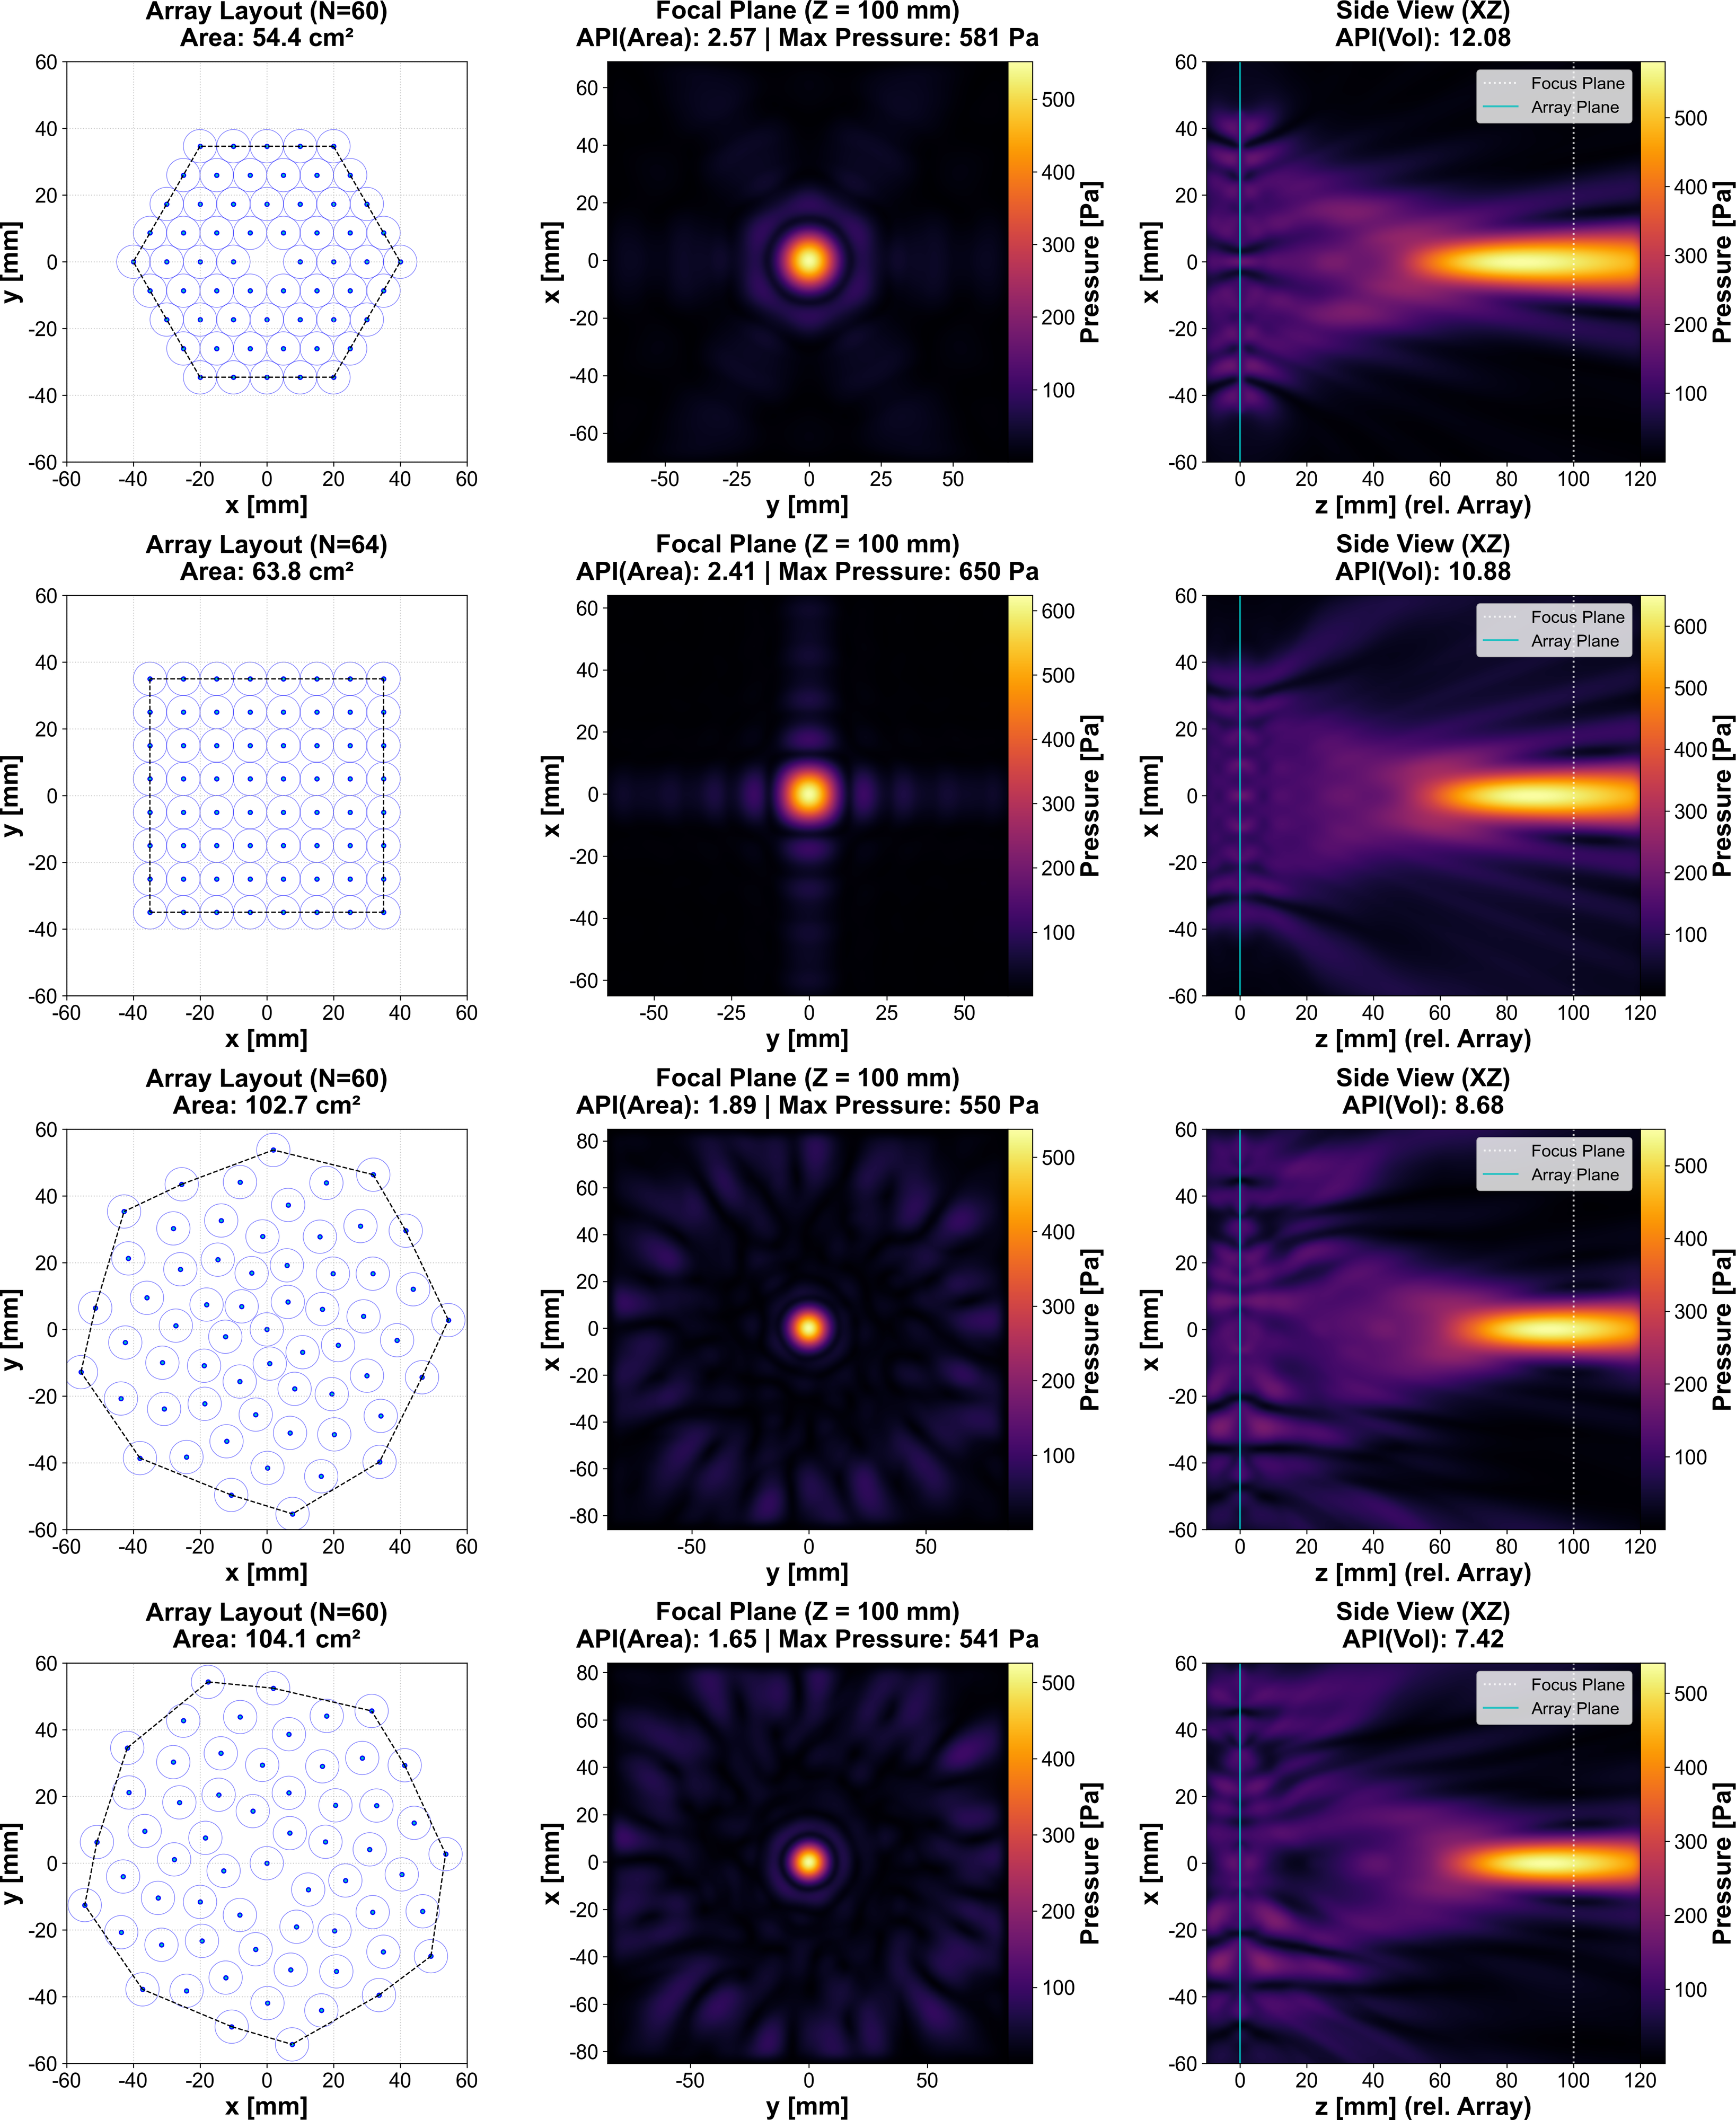
\includegraphics[width=\textwidth]{Figure_Transducer_Array_Arrangement_Focus_Simulation_Results.png}
    \caption{\textbf{Comparative simulation of acoustic focusing performance across different transducer array layouts.} The four rows correspond to (from top to bottom): Hexagonal Close-Packed ($N=60$), Rectangular ($N=64$), Density-Tapered Vogel Spiral ($N=60$), and Optimized Fermat Spiral ($N=60$). The columns display: (Left) The array geometry and physical footprint; (Middle) The normalized acoustic pressure distribution on the focal plane ($z=\qty{100}{\milli\meter}$), annotated with the Area-based Array Performance Index ($\text{API}_{area}$) and maximum pressure; (Right) The side-view pressure distribution in the XZ plane, annotated with the Volume-based Array Performance Index ($\text{API}_{vol}$). The hexagonal array (top row) offers the optimal balance of high pressure output and compact size for the proposed device.}
    \label{fig:supplementary_figure_transducer_array_arrangement_focus_simulation_results}
\end{figure}

We conducted comparative numerical simulations of four distinct phased array configurations to evaluate the acoustic performance of the hexagonal transducer arrangement and explore potential optimizations. The simulation model used the Rayleigh-Sommerfeld integral to calculate the acoustic pressure field generated by circular piston sources ($d=\qty{10}{\milli\meter}$) operating at \qty{40}{\kilo\hertz} in air ($c=\qty{343}{\meter\per\second}$). The configurations included: (1) the proposed Hexagonal Close-Packed (HCP) array ($N=60$, Area=\qty{54.4}{\centi\meter\squared}), (2) a standard Rectangular grid ($N=64$, Area=\qty{63.8}{\centi\meter\squared}), (3) a Density-Tapered Vogel Spiral ($N=60$, Area=\qty{102.7}{\centi\meter\squared}), and (4) an Optimized Fermat Spiral ($N=60$, Area=\qty{104.1}{\centi\meter\squared}).

The geometric arrangement of transducers influences beamforming capabilities. For periodic arrays, the Rectangular layout follows a standard Cartesian grid, while the Hexagonal Close-Packed (HCP) coordinates derive from the triangular lattice vectors defined by:
\begin{equation}
    x_{q,r} = d \left(q + \frac{r}{2}\right), \quad y_{q,r} = d \frac{\sqrt{3}}{2} r
\end{equation}
where $d=\qty{10}{\milli\meter}$ is the pitch and $q, r$ are integers. This hexagonal arrangement maximizes the surface fill factor. In contrast, the aperiodic spiral arrays use the golden angle $\Phi_g = \pi(3-\sqrt{5}) \approx \ang{137.5}$ to suppress grating lobes. The Optimized Fermat Spiral places the $n$-th element at $\theta_n = n \Phi_g$ and radial distance $r_n = c \sqrt{n} (1 + \beta n)$, where $(1 + \beta n)$ introduces a radial density taper to reduce side lobes. The Density-Tapered Vogel Spiral uses an iterative collision-based packing algorithm, where the exclusion radius for the $n$-th element expands linearly as $d_{req}(n) = d_{min}(1 + \alpha n)$, creating a spatially apodized aperture that transitions from a dense core to a sparse periphery.

We quantified focusing performance using the Array Performance Index (API) \cite{priceFibonacciSpiralArranged2018, holmesPostprocessingFullMatrix2005}, defined for both focal area and volume. The area-based API is $\text{API}_{area} = A_{-6dB} / \lambda^2$, where $A_{-6dB}$ represents the area within the \qty{-6}{\decibel} pressure contour on the focal plane. Similarly, the volume-based API is $\text{API}_{vol} = V_{-6dB} / \lambda^3$, capturing the spatial confinement of the acoustic energy. A lower API value indicates sharper focusing and superior diffraction-limited performance.

Spiral configurations demonstrate superior focusing characteristics with significantly lower API values ($\text{API}_{area} \approx 1.65-1.89$) and suppressed grating lobes compared to periodic arrays (\cref{fig:supplementary_figure_transducer_array_arrangement_focus_simulation_results}). However, their sparse arrangement results in a larger physical footprint and reduced peak pressure output ($\approx \qty{540}{\pascal}$) for the same element count. Conversely, the proposed hexagonal array achieves a high peak pressure of \qty{581}{\pascal} with a compact footprint, leveraging the maximum packing density. Although it exhibits characteristic hexagonal grating lobes and a slightly higher API ($\text{API}_{area} = 2.57$), the focal quality remains sufficient for precise tactile stimulation. Consequently, we selected the hexagonal layout for the current prototype to maximize acoustic power density within a handheld form factor, while the spiral designs provide a pathway for future high-fidelity, large-aperture applications.



\SupplementarySection{Psychophysical experiments}
\label{sec:psychophysical_experiments}

\begin{figure}[htbp]
    \centering
    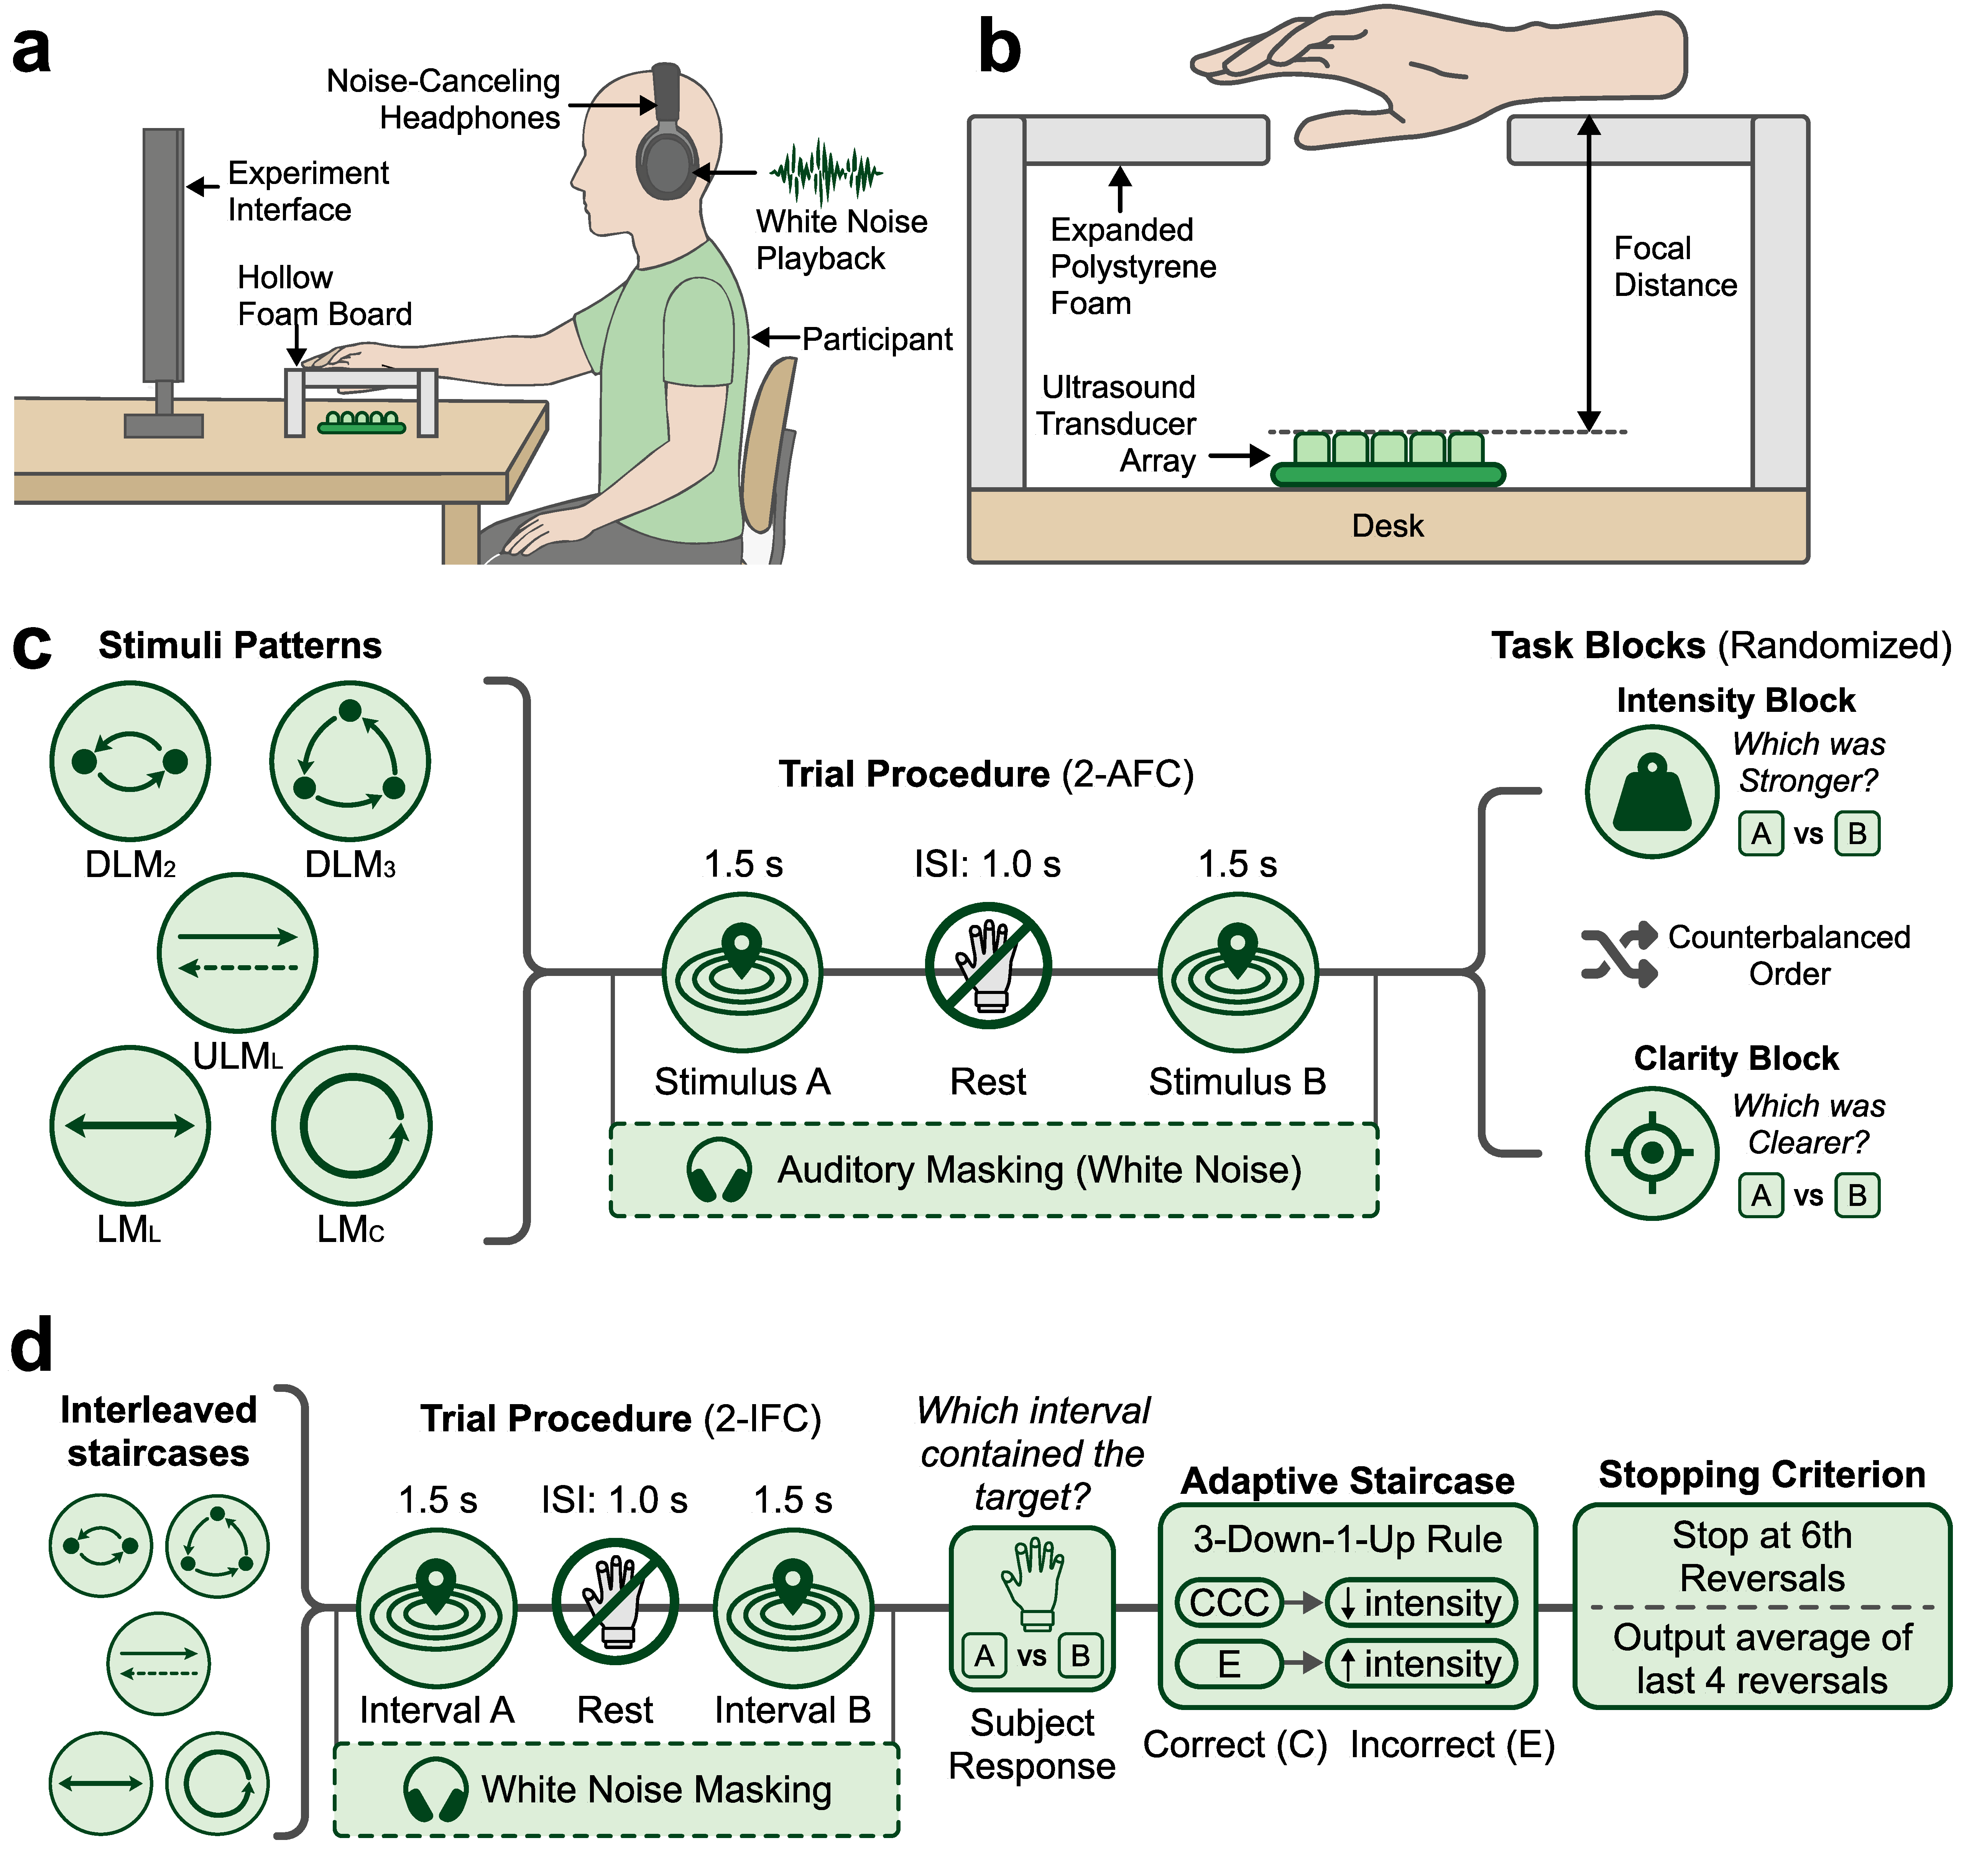
\includegraphics[width=\textwidth]{Figure_Experiment_Scene_and_Procedure.pdf}
    \caption{\textbf{Experimental setup and psychophysical paradigms.} \textbf{a}, Illustration of the experimental environment, showing the participant seated with the palm resting on a fixed hollow foam board, wearing noise-canceling headphones playing white noise to mask auditory cues. \textbf{b}, Cross-sectional view of the acoustic coupling, maintaining a constant focal distance between the transducer array and the glabrous skin. \textbf{c}, Paradigm for Experiment 1 (Relative Preference). Five modulation stimuli (left) were tested using a two-alternative forced-choice (2-AFC) design across separate Intensity and Clarity blocks. \textbf{d}, Paradigm for Experiment 2 (Absolute Detection Threshold). A two-interval forced-choice (2-IFC) task was combined with an interleaved 3-Down-1-Up adaptive staircase to estimate the detection thresholds for each modulation strategy.}
    \label{fig:supplementary_figure_psychophysics_setup}
\end{figure}

The psychophysical evaluation consisted of two complementary experiments sharing the same physical apparatus and acoustic masking controls. Experiment 1 assessed the relative perceptual qualities (intensity and spatial clarity) of five distinct spatiotemporal modulation strategies at a suprathreshold level. Experiment 2 quantified the absolute detection thresholds of these strategies to determine their fundamental perceptual accessibility.

\subsection*{Experiment 1: Relative perceptual dominance (Paired-comparison)}
\label{sec:experiment_1_relative_perceptual_dominance}

Experiment 1 employed a within-participant paired-comparison design to resolve perceptual differences among five ultrasonic spatiotemporal modulation strategies under weak near-threshold tactile conditions. We tested five stimuli: $DLM_2$, $DLM_3$, $ULM_L$, $LM_L$, and $LM_C$, corresponding to two-point discrete lateral modulation, three-point discrete lateral modulation, unidirectional linear lateral modulation, bidirectional linear lateral modulation, and continuous circular lateral modulation. We selected a forced-comparison design because absolute ratings are unstable when the tactile magnitude of individual ultrasonic stimuli is small. Paired judgments provide higher sensitivity for detecting relative perceptual ordering~\citep{bradleyRankAnalysisIncomplete1952, johnsonNeuralBasisHaptic2002}. Thus, the experiment estimated relative perceptual dominance rather than absolute magnitude.

All stimulation used the custom UMH device described above. The carrier frequency was \qty{40}{\kilo\hertz}, and the tactile modulation frequency was fixed at \qty{200}{\hertz}, a range strongly coupled to the Pacinian-dominant vibrotactile channel of glabrous skin~\citep{mountcastleNeuralBasisSense1967, talbotSenseFluttervibrationComparison1968a, johnsonRolesFunctionsCutaneous2001, handlerMechanosensoryNeuronsTouch2021}. Participants placed their palms on a foam support that fixed the hand-device distance and reduced posture-dependent variability in acoustic coupling. They wore noise-cancelling headphones continuously playing white noise so that judgments relied on cutaneous sensation rather than on airborne acoustic leakage or switching sounds. These controls were essential because modulation methods, especially discrete switching conditions, can generate audible artifacts that might otherwise provide non-tactile cues.

The five stimuli were parameterized around a common focal center at $(0,0,\qty{0.1}{\meter})$. The modulation frequency was fixed at $f=\qty{200}{\hertz}$, giving a period of
\begin{equation}
    T = \frac{1}{f} = \qty{5}{\milli\second} .
\end{equation}
Trajectory geometry relied on the assumed cutaneous shear-wave speed $c_s=\qty{5}{\meter\per\second}$ so that focal transition times or scan velocities matched the propagation timescale of surface waves. For $DLM_2$, the focal points lay on a ring of radius $R_{2}=\qty{6.25}{\milli\meter}$, so that the distance between the two diametrically opposed points was $2R_{2}=\qty{12.5}{\milli\meter}=c_sT/2$. For $DLM_3$, the focal points formed an equilateral triangle on a ring of radius $R_{3}=\qty{4.81}{\milli\meter}$, such that the adjacent-point spacing satisfied $\sqrt{3}R_{3}\approx \qty{8.33}{\milli\meter}=c_sT/3$. For $ULM_L$, the focus traversed a unidirectional linear path of length $L_{U}=\qty{30}{\milli\meter}$ in each period, yielding an effective scan speed
\begin{equation}
    v_U = \frac{L_U}{T} = \qty{6}{\meter\per\second} \approx 1.2\,c_s .
\end{equation}
For $LM_L$, the focus moved bidirectionally between two endpoints separated by \qty{15}{\milli\meter}. Because the focus covered the outbound and return paths within one modulation period, the total travelled distance per period was \qty{30}{\milli\meter}, again corresponding to an average path speed of \qty{6}{\meter\per\second}. For $LM_C$, the focus moved continuously along a circular trajectory of radius $R_C=\qty{4.77}{\milli\meter}$, for which the tangential speed was set to the same Mach number regime, $v_C\approx \qty{6}{\meter\per\second} \approx 1.2\,c_s$. Matching the nominal kinematic scale across conditions reduced confounding by trivial differences in scan frequency or gross path length and focused the comparison on how different spatiotemporal wave organizations shape perception.

The experiment contained two task blocks. In the Intensity block, participants reported which of two successively presented stimuli felt stronger. In the Spatial block, participants reported which stimulus felt smaller or clearer as a tactile point. We retained the label ``smaller / clearer'' because the task captured the perceptual sharpness of a localized tactile percept under weak ultrasonic stimulation, rather than physical spatial acuity in the strict classical two-point-discrimination sense. Under near-threshold conditions, judgments of ``clarity'' likely integrate perceived detectability, compactness, temporal stability, and confidence in addition to apparent stimulus area.

We randomized the order of the two task blocks for each participant. Within each block, the five stimuli generate $\binom{5}{2}=10$ unordered pairs. To control for first-versus-second presentation effects, every unordered pair was presented in both temporal orders, yielding $5\times4=20$ ordered trials per block. The trial list was therefore the complete set of ordered permutations of length two over the five stimuli. Trial order was then shuffled independently within each block. Because the block order was also randomized, each participant completed a total of 40 forced-choice trials. During data collection, the graphical user interface concealed the identities of the current stimulus pair from both participant and experimenter, implementing an operationally blind procedure.

Each trial followed a fixed temporal structure. Stimulus A was presented for \qty{1.5}{\second}, followed by a silent interval of \qty{1.0}{\second}, after which Stimulus B was presented for \qty{1.5}{\second}. The silent interval reduced immediate peripheral and central carry-over while keeping the comparison in short-term tactile memory. Replay was not allowed. Participants had to commit to a first-pass comparative judgment, consistent with standard two-alternative forced-choice logic to avoid strategic averaging across repeated presentations~\citep{bradleyRankAnalysisIncomplete1952}. The response was recorded only after the second stimulus ended. Reaction time was measured from the offset of Stimulus B to the submission of the response, so the decision time indexed post-stimulus comparative evaluation rather than motor latency.

Responses were stored trial-by-trial in comma-separated files. Each record contained the participant identifier, timestamp, block index, block type, trial number, stimulus identity in the first and second positions, the selected winner, and reaction time. Because each block queried only one perceptual dimension, the non-relevant response field for that trial was left empty. This structure preserved the full order information required for paired-comparison modeling while keeping intensity and spatial judgments analytically separable.

A priori sample-size estimation in G*Power (effect size $g=0.2$, $\alpha=0.05$, power $=0.8$, constant proportion $=0.5$) yielded a required sample size of 49 paired observations at the comparison level. Since each participant contributed both presentation orders for a given unordered pair, this required approximately 25 participants. We recruited 30 participants (15 male, 15 female, mean age $24.17 \pm 1.61$ years) to provide a margin against data loss and to stabilize estimation of individual differences in the mixed-effects analysis.

The primary analysis treated paired choices as comparative preference data and modeled them with a Bayesian mixed-effects Bradley--Terry framework~\citep{bradleyRankAnalysisIncomplete1952}. For each block, we converted the raw trial table into long format, with one row per valid paired comparison. Let stimuli $i$ and $j$ denote the first and second members of a presented pair for a given trial, and let $Y_{n}=1$ if stimulus $i$ was chosen over stimulus $j$ on trial $n$, and $Y_{n}=0$ otherwise. The probability that stimulus $i$ defeats stimulus $j$ is:
\begin{equation}
    \Pr(Y_n=1)=\frac{\exp\left(\lambda_i-\lambda_j+b_{p[n]}\right)}{1+\exp\left(\lambda_i-\lambda_j+b_{p[n]}\right)} ,
\end{equation}
where $\lambda_i$ and $\lambda_j$ are fixed-effect latent scores for the two modulation methods and $b_{p[n]}$ is the participant-specific random intercept. We estimated the model using a binomial Bayesian mixed generalized linear model. After fitting, we mean-centered the estimated method scores:
\begin{equation}
    \tilde{\lambda}_i = \lambda_i - \frac{1}{K}\sum_{k=1}^{K}\lambda_k,
\end{equation}
where $K=5$ is the number of modulation methods. This zero-centered representation preserves all pairwise contrasts while making the average method score equal to zero, simplifying visual comparison.

We constructed a win matrix for each block to provide an intuitive summary of pairwise dominance. However, inferential conclusions relied on the mixed-effects Bradley--Terry estimates and their covariance. We evaluated pairwise contrasts between methods using Wald statistics derived from the fitted score covariance matrix. For a contrast between methods $i$ and $j$:
\begin{equation}
    \Delta_{ij}=\tilde{\lambda}_i-\tilde{\lambda}_j,
    \qquad
    z_{ij}=\frac{\Delta_{ij}}{\sqrt{\mathrm{Var}(\Delta_{ij})}},
\end{equation}
with two-sided $p$ values obtained from the standard normal distribution. We also report the corresponding odds ratio,
\begin{equation}
    \mathrm{OR}_{ij}=\exp(\Delta_{ij}),
\end{equation}
which quantifies the multiplicative advantage of method $i$ over method $j$ in the paired-comparison choice probability.

We analyzed decision time as a secondary marker of discriminability. Longer decisions indicated smaller perceptual distances between the two methods. We excluded reaction times shorter than \qty{0.2}{\second} or longer than \qty{10}{\second}. For the remaining trials, we log-transformed raw reaction time $RT$:
\begin{equation}
    \mathrm{LogRT}=\ln(RT),
\end{equation}
and then standardized within participant to remove idiosyncratic baseline response speed:
\begin{equation}
    Z\mathrm{LogRT}_{n}=\frac{\mathrm{LogRT}_{n}-\mu_{p[n]}}{\sigma_{p[n]}} ,
\end{equation}
where $\mu_{p[n]}$ and $\sigma_{p[n]}$ are the participant-specific mean and standard deviation of log reaction time. We averaged $Z\mathrm{LogRT}$ across all presentations of each unordered stimulus pair to form a symmetric reaction-time matrix. Darker values indicate longer normalized decisions and smaller perceptual separation.

Visualization followed the statistical analysis structure. For Intensity and Spatial blocks, each method was displayed as a bar representing the centered Bradley--Terry score, with error bars corresponding to the \qty{95}{\percent} confidence interval. We marked significant pairwise contrasts directly on the plots. Reaction-time results were summarized as a stimulus-by-stimulus heat map of mean standardized log reaction time.

In the Intensity block, $ULM_L$ achieved the highest centered Bradley--Terry score ($0.74\pm0.11$), followed by $DLM_2$ ($0.34\pm0.11$), $DLM_3$ ($-0.04\pm0.11$), $LM_C$ ($-0.18\pm0.11$), and $LM_L$ ($-0.86\pm0.12$). $ULM_L$ was significantly preferred over every other method, and $LM_L$ performed worst overall. In the Spatial block, $ULM_L$ again showed the highest score ($0.24\pm0.10$), followed by $DLM_2$ ($0.11\pm0.10$), $DLM_3$ ($-0.04\pm0.10$), $LM_C$ ($-0.08\pm0.10$), and $LM_L$ ($-0.23\pm0.10$). However, spatial judgments were less strongly separated than intensity judgments. Reaction-time analysis showed that decisions were slowest for pairs such as $DLM_3$ versus $LM_C$ and $ULM_L$ versus $DLM_2$, consistent with their close perceptual proximity. By contrast, comparisons involving $LM_L$ were typically faster, consistent with its poor perceptual performance.

Beyond merely reflecting task difficulty, shorter reaction times (Z-Log-RT) in high-performing conditions (like comparisons against $LM_L$) suggest that participants received neural signals with high signal-to-noise ratios (SNR). In the case of $ULM_L$, despite its physically smoother spatial gradient, the rapid decision times observed when distinguishing it from poorer stimuli (e.g., $LM_L$) indicate that its high spatiotemporal coherence generates a distinct and reliable neural representation. This ``decision confidence'' aligns with the subjective reports of spatial clarity, suggesting that the perception of a ``clear point'' is driven by the temporal certainty of the neural train rather than static spatial contrast.

These psychophysical observations informed the mechanistic interpretation. Perceptual superiority did not follow simple expectations based on static focal intensity or geometric sharpness. Instead, the best-performing condition preserved the intended \qty{200}{\hertz} temporal structure while organizing cutaneous shear-wave propagation into a coherent spatiotemporal pattern. The psychophysical protocol thus provided a sensitive behavioral assay of how modulation-dependent wave organization shapes tactile perception.

\subsection*{Experiment 2: Absolute detection thresholds (Adaptive staircase)}
\label{sec:experiment_2_absolute_detection_thresholds}

Experiment 2 measured the absolute detection thresholds of the five modulation strategies ($DLM_2$, $DLM_3$, $ULM_L$, $LM_L$, and $LM_C$). While Experiment 1 evaluated relative perceptual dominance at a fixed suprathreshold level, Experiment 2 determined the minimum acoustic output required for reliable perception. We employed a two-interval forced-choice (2-IFC) task combined with an interleaved adaptive staircase procedure~\citep{leekAdaptiveProceduresPsychophysical2001} (\cref{fig:supplementary_figure_psychophysics_setup}d).

We tested the five modulation conditions concurrently using randomly interleaved staircases. This strategy distributed time-dependent confounding factors---such as tactile adaptation, fatigue, and fluctuations in attention---evenly across all conditions. Spatial trajectories and the \qty{200}{\hertz} modulation frequency matched Experiment 1.

Each trial followed a standard 2-IFC temporal structure with two \qty{1.5}{\second} observation intervals separated by a \qty{1.0}{\second} silent gap. Only one interval contained the stimulus; the other was blank. Assignment was randomized. Participants made a forced-choice judgment indicating which interval contained the stimulus. This paradigm eliminates subjective criterion bias, grounding the threshold estimate in objective performance relative to a \qty{50}{\percent} chance level.

A transformed 3-Down-1-Up staircase rule~\citep{levittTransformedUpdownMethods1971} adjusted stimulus intensity. Intensity decreased by one step after three consecutive correct responses and increased by one step after a single incorrect response. This rule converges asymptotically to a stimulus level corresponding to a \qty{79.4}{\percent} probability of correct detection~\citep{levittTransformedUpdownMethods1971, garcia-perezForcedchoiceStaircasesFixed1998a}.

Crucially, we parameterized staircase steps in physically calibrated normalized intensity space ($I_{\mathrm{norm}}$) to ensure equal perceptual step sizes. Based on the hardware transfer function, we constructed a discrete stimulus grid with a base intensity step of $\Delta I = 0.08$. The corresponding hardware strength command $S$ was computed via the inverse mapping:
\begin{equation}
    S(I_{\mathrm{norm}}) = \frac{200}{\pi} \arcsin\left(\sqrt{I_{\mathrm{norm}}}\right).
\end{equation}
Each staircase was initialized at a highly perceptible level ($S = 80$). We used a variable step-size strategy: the staircase began with a coarse step of $2\Delta I$ ($0.16$), reducing to $1\Delta I$ ($0.08$) after the first two reversals.

A staircase terminated after 6 reversals (minimum 10 trials, maximum 40 trials). We calculated the absolute detection threshold as the arithmetic mean of the stimulus intensities at the final 4 reversals. Physical environmental controls (fixed hand-to-array distance, noise-canceling headphones) matched Experiment 1.

The absolute detection thresholds, expressed in terms of normalized acoustic intensity ($I_{\mathrm{norm}}$), revealed consistent differences among the modulation strategies, corroborating the suprathreshold preference findings from Experiment 1. A lower threshold indicates higher perceptual efficiency. $ULM_L$ exhibited the lowest mean detection threshold ($0.281 \pm 0.040$, mean $\pm$ SEM), followed by $DLM_2$ ($0.313 \pm 0.040$), $DLM_3$ ($0.316 \pm 0.039$), and $LM_C$ ($0.347 \pm 0.047$). In contrast, the traditional bidirectional linear scan ($LM_L$) required the highest acoustic output to be detected ($0.371 \pm 0.040$).

A Friedman test indicated a marginally significant overall effect of modulation strategy on the detection threshold ($p = 0.0588$). Post-hoc pairwise comparisons with Holm--Bonferroni correction confirmed that the threshold for $ULM_L$ was significantly lower than that for $LM_L$ ($p = 0.003$). Similarly, $DLM_2$ demonstrated a significantly lower threshold compared to $LM_L$ ($p = 0.030$). Although $ULM_L$ maintained the lowest absolute threshold numerically, its differences with $DLM_2$, $DLM_3$, and $LM_C$ did not reach statistical significance in this absolute detection paradigm.

These results provide strong cross-validation for the hypothesized mechanism. $ULM_L$, which generated the weakest local physical extremes but the highest spatiotemporal coherence, proved to be the most efficient stimulus near the absolute threshold of perception. This indicates that $ULM_L$ maximizes the conversion of mechanical energy into neural action potentials through coherent integration, rather than relying on instantaneous high-pressure extremes. Furthermore, the poor performance of $LM_L$ in both subjective intensity (Experiment 1) and absolute detection (Experiment 2) quantitatively demonstrates that its inherent frequency doubling effect (shifting energy from the optimal \qty{200}{\hertz} band to \qty{400}{\hertz} and higher harmonics) leads to substantial energy waste and degraded perception. $DLM_2$ also performed efficiently, suggesting that appropriate discrete spatial hopping can effectively evade destructive interference and maintain high perceptual efficacy.

\SupplementarySection{Numerical Simulation of Tactile Wave Propagation}
\label{sec:numerical_simulation_tactile_wave_propagation}

To resolve how different ultrasonic spatiotemporal modulation strategies reorganize mechanically relevant wave propagation within soft tissue, we performed three-dimensional elastodynamic simulations using the k-Wave pseudo-spectral time-domain elastic solver \texttt{pstdElastic3D} in MATLAB. The simulated tissue block occupied a Cartesian domain of \qtyproduct{80 x 80 x 40}{\milli\meter}, discretized on a uniform grid with
\begin{equation}
    \Delta x = \Delta y = \Delta z = \qty{1.0}{\milli\meter},
\end{equation}
yielding $N_x=N_y=80$ and $N_z=40$ grid points. Time integration used a Courant--Friedrichs--Lewy factor of $\mathrm{CFL}=0.3$. The temporal step was:
\begin{equation}
    \Delta t = \mathrm{CFL}\frac{\Delta x}{c_{p,\mathrm{sim}}},
\end{equation}
With $c_{p,\mathrm{sim}}=\qty{100}{\meter\per\second}$, $\Delta t=\qty{3}{\micro\second}$. The modulation frequency was fixed at
\begin{equation}
    f_0 = \qty{200}{\hertz},
    \qquad
    T = \frac{1}{f_0} = \qty{5}{\milli\second},
\end{equation}
and total simulation duration was 15 modulation cycles,
\begin{equation}
    t_{\mathrm{sim}} = 15T = \qty{75}{\milli\second},
\end{equation}

The medium was modeled as homogeneous, isotropic, and linearly elastic with frequency-dependent attenuation. Material parameters were density $\rho=\qty{923.5}{\kilo\gram\per\cubic\meter}$, shear-wave speed $c_s=\qty{5.0}{\meter\per\second}$, and simulated compressional-wave speed $c_{p,\mathrm{sim}}=\qty{100}{\meter\per\second}$. The shear modulus was:
\begin{equation}
    G = \rho c_s^2,
\end{equation}
giving $G\approx \qty{23.1}{\kilo\pascal}$. We used the reduced $c_{p,\mathrm{sim}}$ for time stepping to preserve the scale separation $c_{p,\mathrm{sim}} \gg c_s$ while reducing computational burden. This approximation is appropriate because the objective was to isolate the slower lateral shear-wave dynamics that dominate tactile spatiotemporal structure.

Attenuation followed frequency power laws,
\begin{equation}
    \alpha_p(f) = \alpha_{p0} f^{y_p},
    \qquad
    \alpha_s(f) = \alpha_{s0} f^{y_s},
\end{equation}
with $\alpha_{p0}=\qty{0.1}{\decibel\per\mega\hertz\tothe{1.5}\per\centi\meter}$, $y_p=1.5$, $\alpha_{s0}=\qty{10}{\decibel\per\mega\hertz\squared\per\centi\meter}$, and $y_s=2.0$. To approximate a mechanically semi-infinite substrate, we used external perfectly matched layers (\texttt{PMLSize}$=[20,20,10]$). We added a quadratic sponge layer to the lower part of the domain:
\begin{equation}
    \alpha_{\mathrm{sponge}}(k)=\alpha_{\max}\left(\frac{k-1}{N_{\mathrm{sponge}}-1}\right)^2,
    \qquad k=1,\dots,N_{\mathrm{sponge}},
\end{equation}
with $N_{\mathrm{sponge}}=20$ and $\alpha_{\max}=30$. This ensured that observed lateral wave patterns arose from imposed modulation trajectories rather than reverberation.

The excitation was a normal stress source on the top surface ($z=0$):
\begin{equation}
    S_{zz}(x,y,t) = -S_0 \exp\!\left[-\frac{(x-x_f(t))^2+(y-y_f(t))^2}{2\sigma^2}\right],
\end{equation}
with $S_0=\qty{100}{\pascal}$ and $\sigma=\qty{4.25}{\milli\meter}$. The \qty{200}{\hertz} temporal structure arose entirely from the periodic motion of the focal center $(x_f(t),y_f(t))$.

The five stimulation conditions reproduced the trajectory definitions from Experiment 1. For discrete lateral modulation, the focus jumped among equally spaced points on a circle. If a modulation cycle was divided into $N$ equal phase sectors, the active point index was:
\begin{equation}
    n(t)=\left\lfloor N\frac{\mathrm{mod}(t,T)}{T}\right\rfloor+1,
\end{equation}
and the focal coordinates were:
\begin{equation}
    x_f(t)=R\cos\theta_{n(t)},
    \qquad
    y_f(t)=R\sin\theta_{n(t)},
    \qquad
    \theta_n = (n-1)\frac{2\pi}{N}.
\end{equation}
For $DLM_2$ ($N=2$, $R=\qty{6.25}{\milli\meter}$):
\begin{equation}
    d_{\mathrm{DLM_2}} = 2R = \qty{12.5}{\milli\meter} = c_s\frac{T}{2}.
\end{equation}
For $DLM_3$ ($N=3$, $R=\qty{4.81}{\milli\meter}$):
\begin{equation}
    d_{\mathrm{DLM_3}} = \sqrt{3}R \approx \qty{8.33}{\milli\meter} \approx c_s\frac{T}{3}.
\end{equation}
These relations matched shear-wave travel distance to actuation site spacing.

For continuous scanning, the focus moved along line or circle trajectories. In $ULM_L$ ($L=\qty{30}{\milli\meter}$):
\begin{equation}
    x_f(t) = -\frac{L}{2}+L\frac{\mathrm{mod}(t,T)}{T},
    \qquad
    y_f(t)=0,
\end{equation}
The scan speed was:
\begin{equation}
    v_{\mathrm{ULM}} = \frac{L}{T} = \qty{6}{\meter\per\second} \approx 1.2 c_s.
\end{equation}
For $LM_L$ ($L=\qty{15}{\milli\meter}$):
\begin{equation}
    x_f(t)=
    \begin{cases}
        -\dfrac{L}{2}+L\dfrac{\phi(t)}{0.5},    & \phi(t)<0.5,    \\[6pt]
        \dfrac{L}{2}-L\dfrac{\phi(t)-0.5}{0.5}, & \phi(t)\ge 0.5,
    \end{cases}
    \qquad
    y_f(t)=0,
\end{equation}
where $\phi(t)=\mathrm{mod}(t,T)/T$. The total distance traveled per cycle was \qty{30}{\milli\meter} (average speed \qty{6}{\meter\per\second}). For $LM_C$ ($R=\qty{4.77}{\milli\meter}$):
\begin{equation}
    x_f(t)=R\cos\bigl(2\pi\phi(t)\bigr),
    \qquad
    y_f(t)=R\sin\bigl(2\pi\phi(t)\bigr),
\end{equation}
Tangential velocity was:
\begin{equation}
    v_{\mathrm{LM_C}}=\frac{2\pi R}{T}\approx \qty{6.0}{\meter\per\second},
\end{equation}
placing all moving-focus conditions in a matched velocity regime.

The solver recorded the stress tensor and displacement field on an analysis plane at \qty{1}{\milli\meter} depth. We constructed the instantaneous shear-stress magnitude:
\begin{equation}
    |\boldsymbol{\tau}|(x,y,t)=\sqrt{\tau_{xy}^2(x,y,t)+\tau_{xz}^2(x,y,t)+\tau_{yz}^2(x,y,t)}.
\end{equation}

To compare modulation conditions, we evaluated steady-state metrics over the final modulation cycle ($\Omega_{\mathrm{ss}}$). Root-mean-square shear magnitude was:
\begin{equation}
    \tau_{\mathrm{RMS}}(x,y)=\sqrt{\frac{1}{|\Omega_{\mathrm{ss}}|}\sum_{t\in\Omega_{\mathrm{ss}}}|\boldsymbol{\tau}(x,y,t)|^2},
\end{equation}
Peak stress map:
\begin{equation}
    \tau_{\mathrm{peak}}(x,y)=\max_t |\boldsymbol{\tau}(x,y,t)|,
\end{equation}
Maximum rate of change:
\begin{equation}
    \dot{\tau}_{\mathrm{peak}}(x,y)=\max_t \left|\frac{\partial |\boldsymbol{\tau}(x,y,t)|}{\partial t}\right|,
\end{equation}
This metric captures dynamic impact.

Spatial sharpness was quantified from the gradient at the final time $t_{\mathrm{end}}$ (\cref{fig:supplementary_figure_sim_1_full_spatial}):
\begin{equation}
    \nabla |\boldsymbol{\tau}|(x,y,t_{\mathrm{end}})=
    \left(
    \frac{\partial |\boldsymbol{\tau}|}{\partial x},
    \frac{\partial |\boldsymbol{\tau}|}{\partial y}
    \right),
\end{equation}
\begin{equation}
    G_{\tau}(x,y)=\sqrt{\left(\frac{\partial |\boldsymbol{\tau}|}{\partial x}\right)^2+
        \left(\frac{\partial |\boldsymbol{\tau}|}{\partial y}\right)^2}.
\end{equation}

\begin{figure}[htbp]
    \centering
    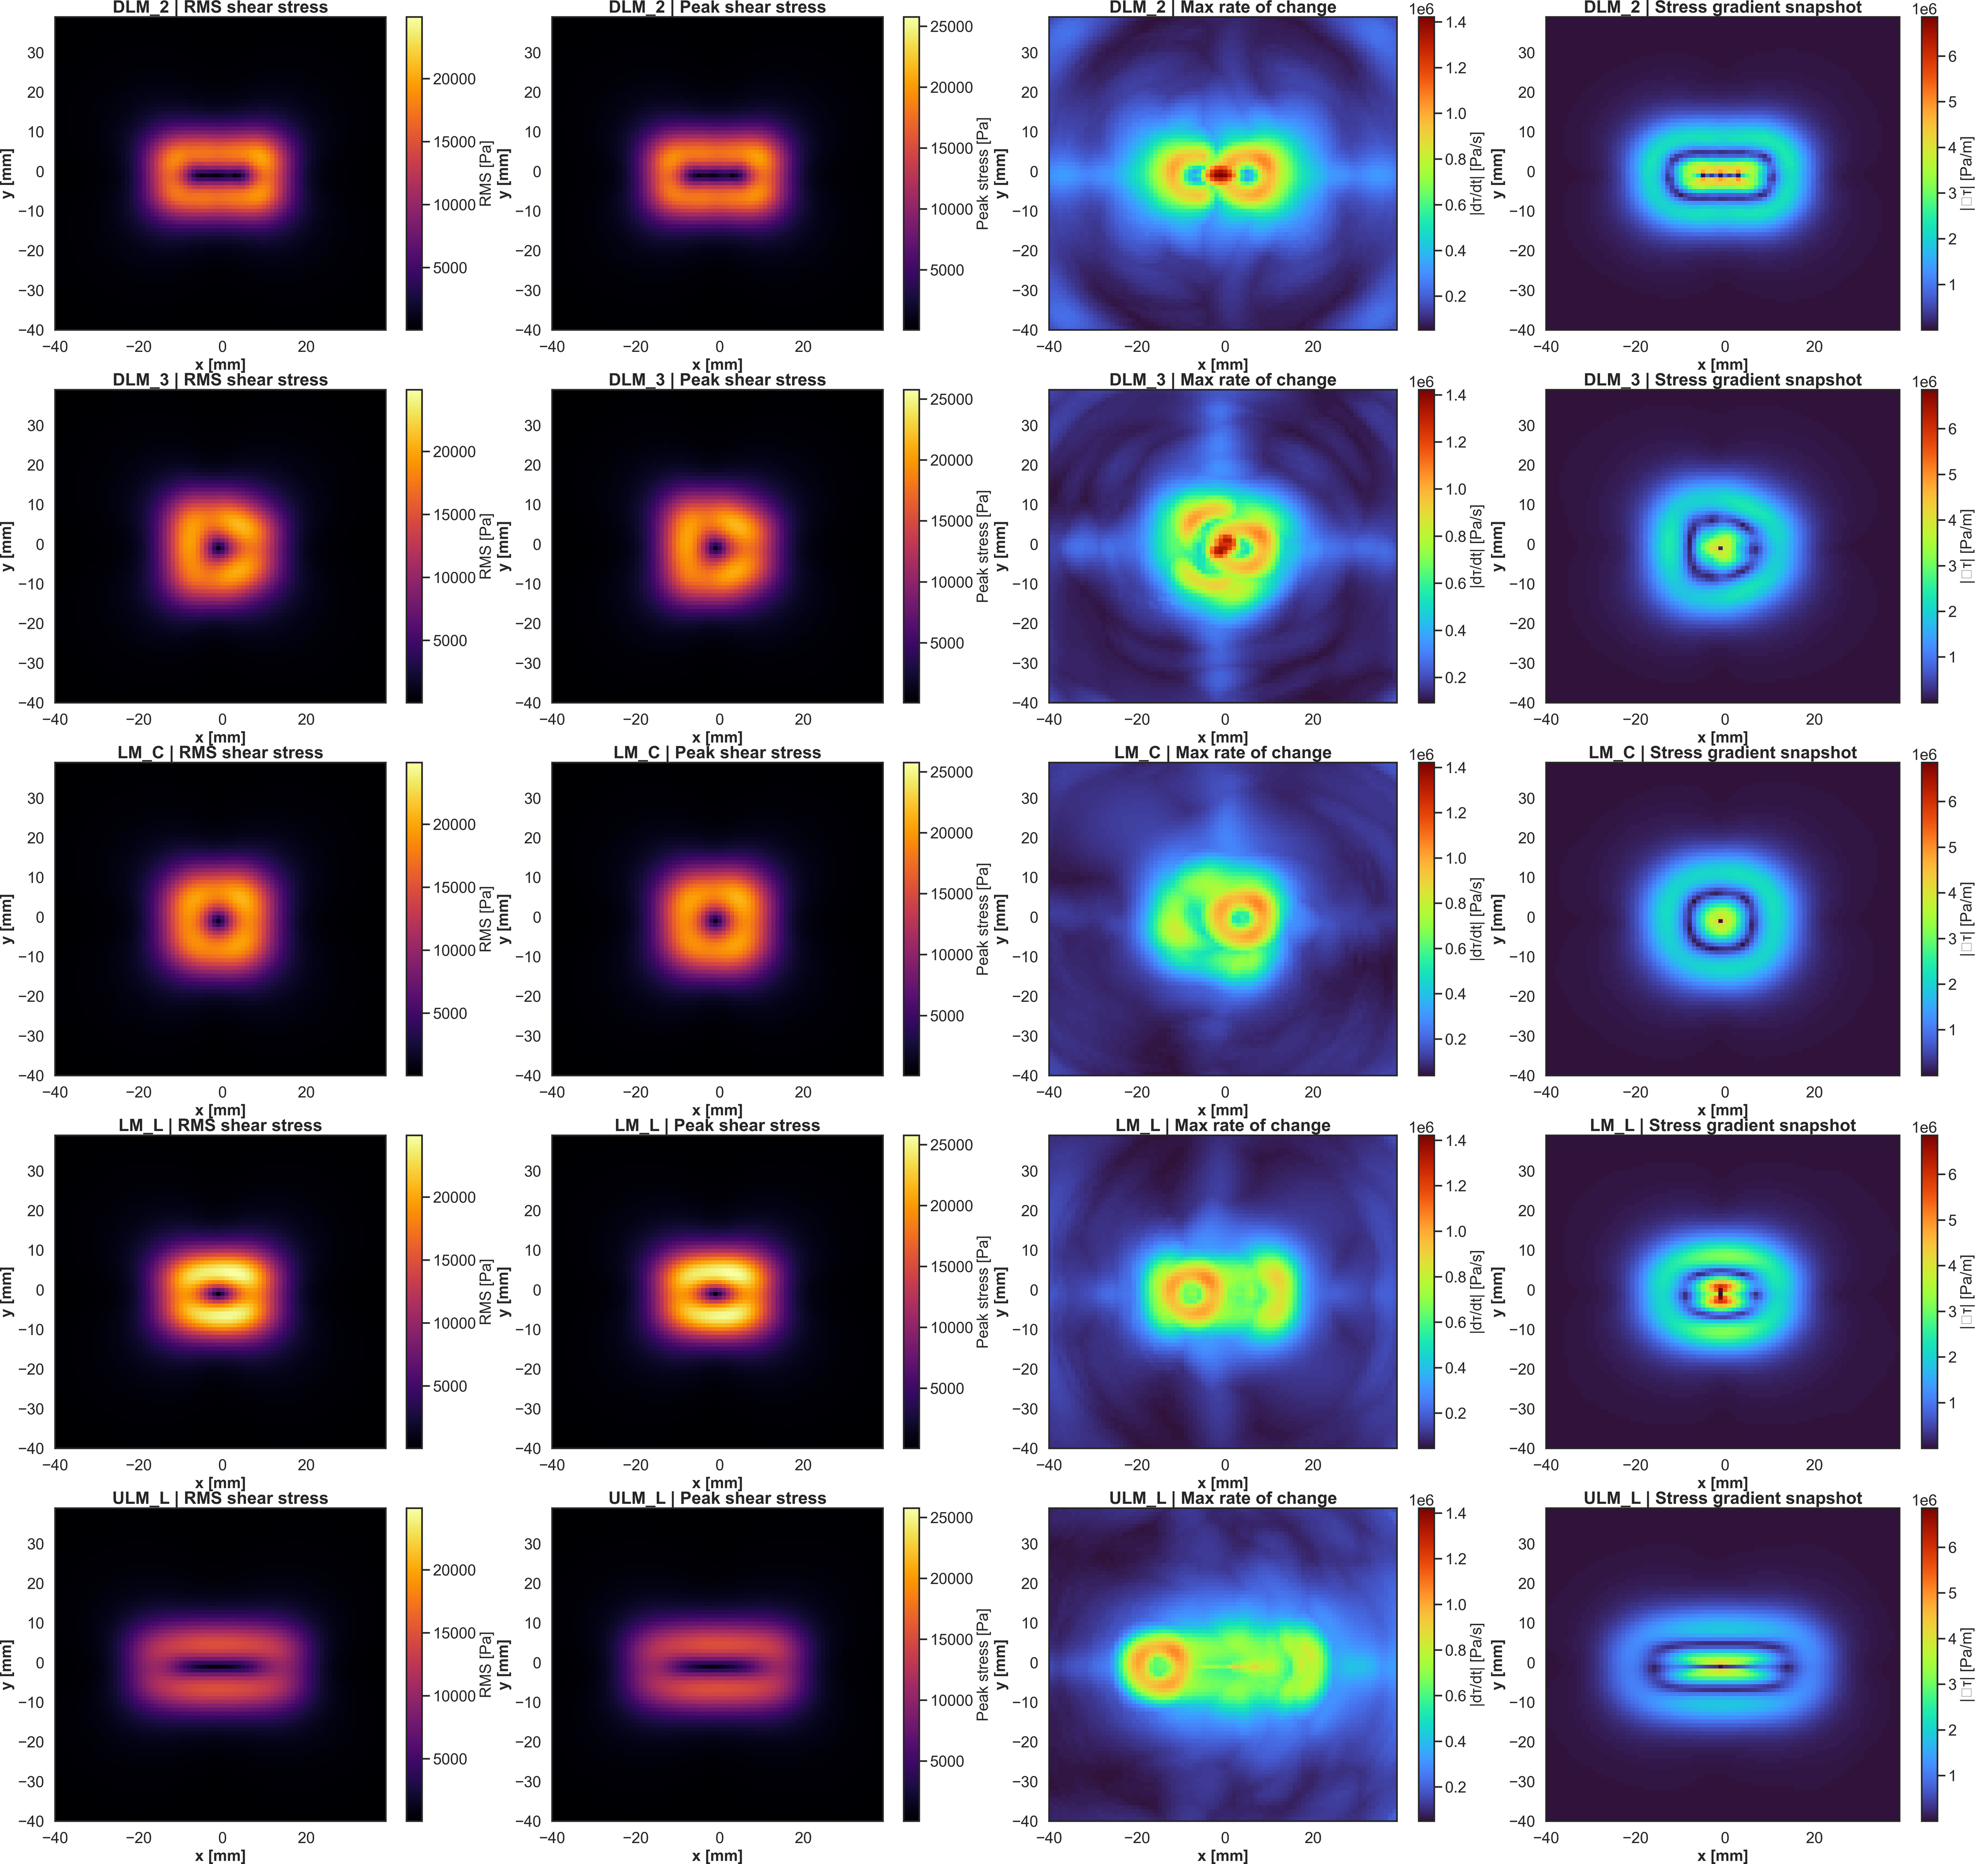
\includegraphics[width= \textwidth]{Figure_Sim_1_Full_Spatial.png}
    \caption{\textbf{Spatial distribution of stress metrics for different modulation schemes.} The rows correspond to the five modulation methods: DLM-2, DLM-3, LM-C, LM-L, and ULM-L. The columns display, from left to right: (1) \textbf{RMS Shear Stress}: The root-mean-square magnitude of the shear stress, indicating the time-averaged energy distribution. (2) \textbf{Peak Shear Stress}: The maximum instantaneous stress magnitude recorded. (3) \textbf{Max Rate of Change}: The maximum time derivative of the stress ($\max |d\boldsymbol{\tau}/dt|$), representing the dynamic impact intensity. (4) \textbf{Stress Gradient Snapshot}: A snapshot of the spatial stress gradient magnitude ($|\nabla \boldsymbol{\tau}|$), reflecting the spatial sharpness of the stimulus. All metrics are evaluated at a depth of \qty{1}{\milli\meter}.}
    \label{fig:supplementary_figure_sim_1_full_spatial}
\end{figure}

We characterized temporal structure using the center waveform:
\begin{equation}
    w_c(t)=|\boldsymbol{\tau}(0,0,t)|,
\end{equation}
and an $x$--$t$ diagram along the midline:
\begin{equation}
    X_{\tau}(x,t)=\tau_{xz}(x,0,t).
\end{equation}
Wavefront snapshots of $\tau_{xy}$ and $u_z$ at four times within the first cycle:
\begin{equation}
    t_k \in \left\{\frac{T}{4},\frac{T}{2},\frac{3T}{4},T\right\},
\end{equation}
allowed inspection of propagation geometry (\cref{fig:supplementary_figure_sim_1_full_temporal}).

\begin{figure}[htbp]
    \centering
    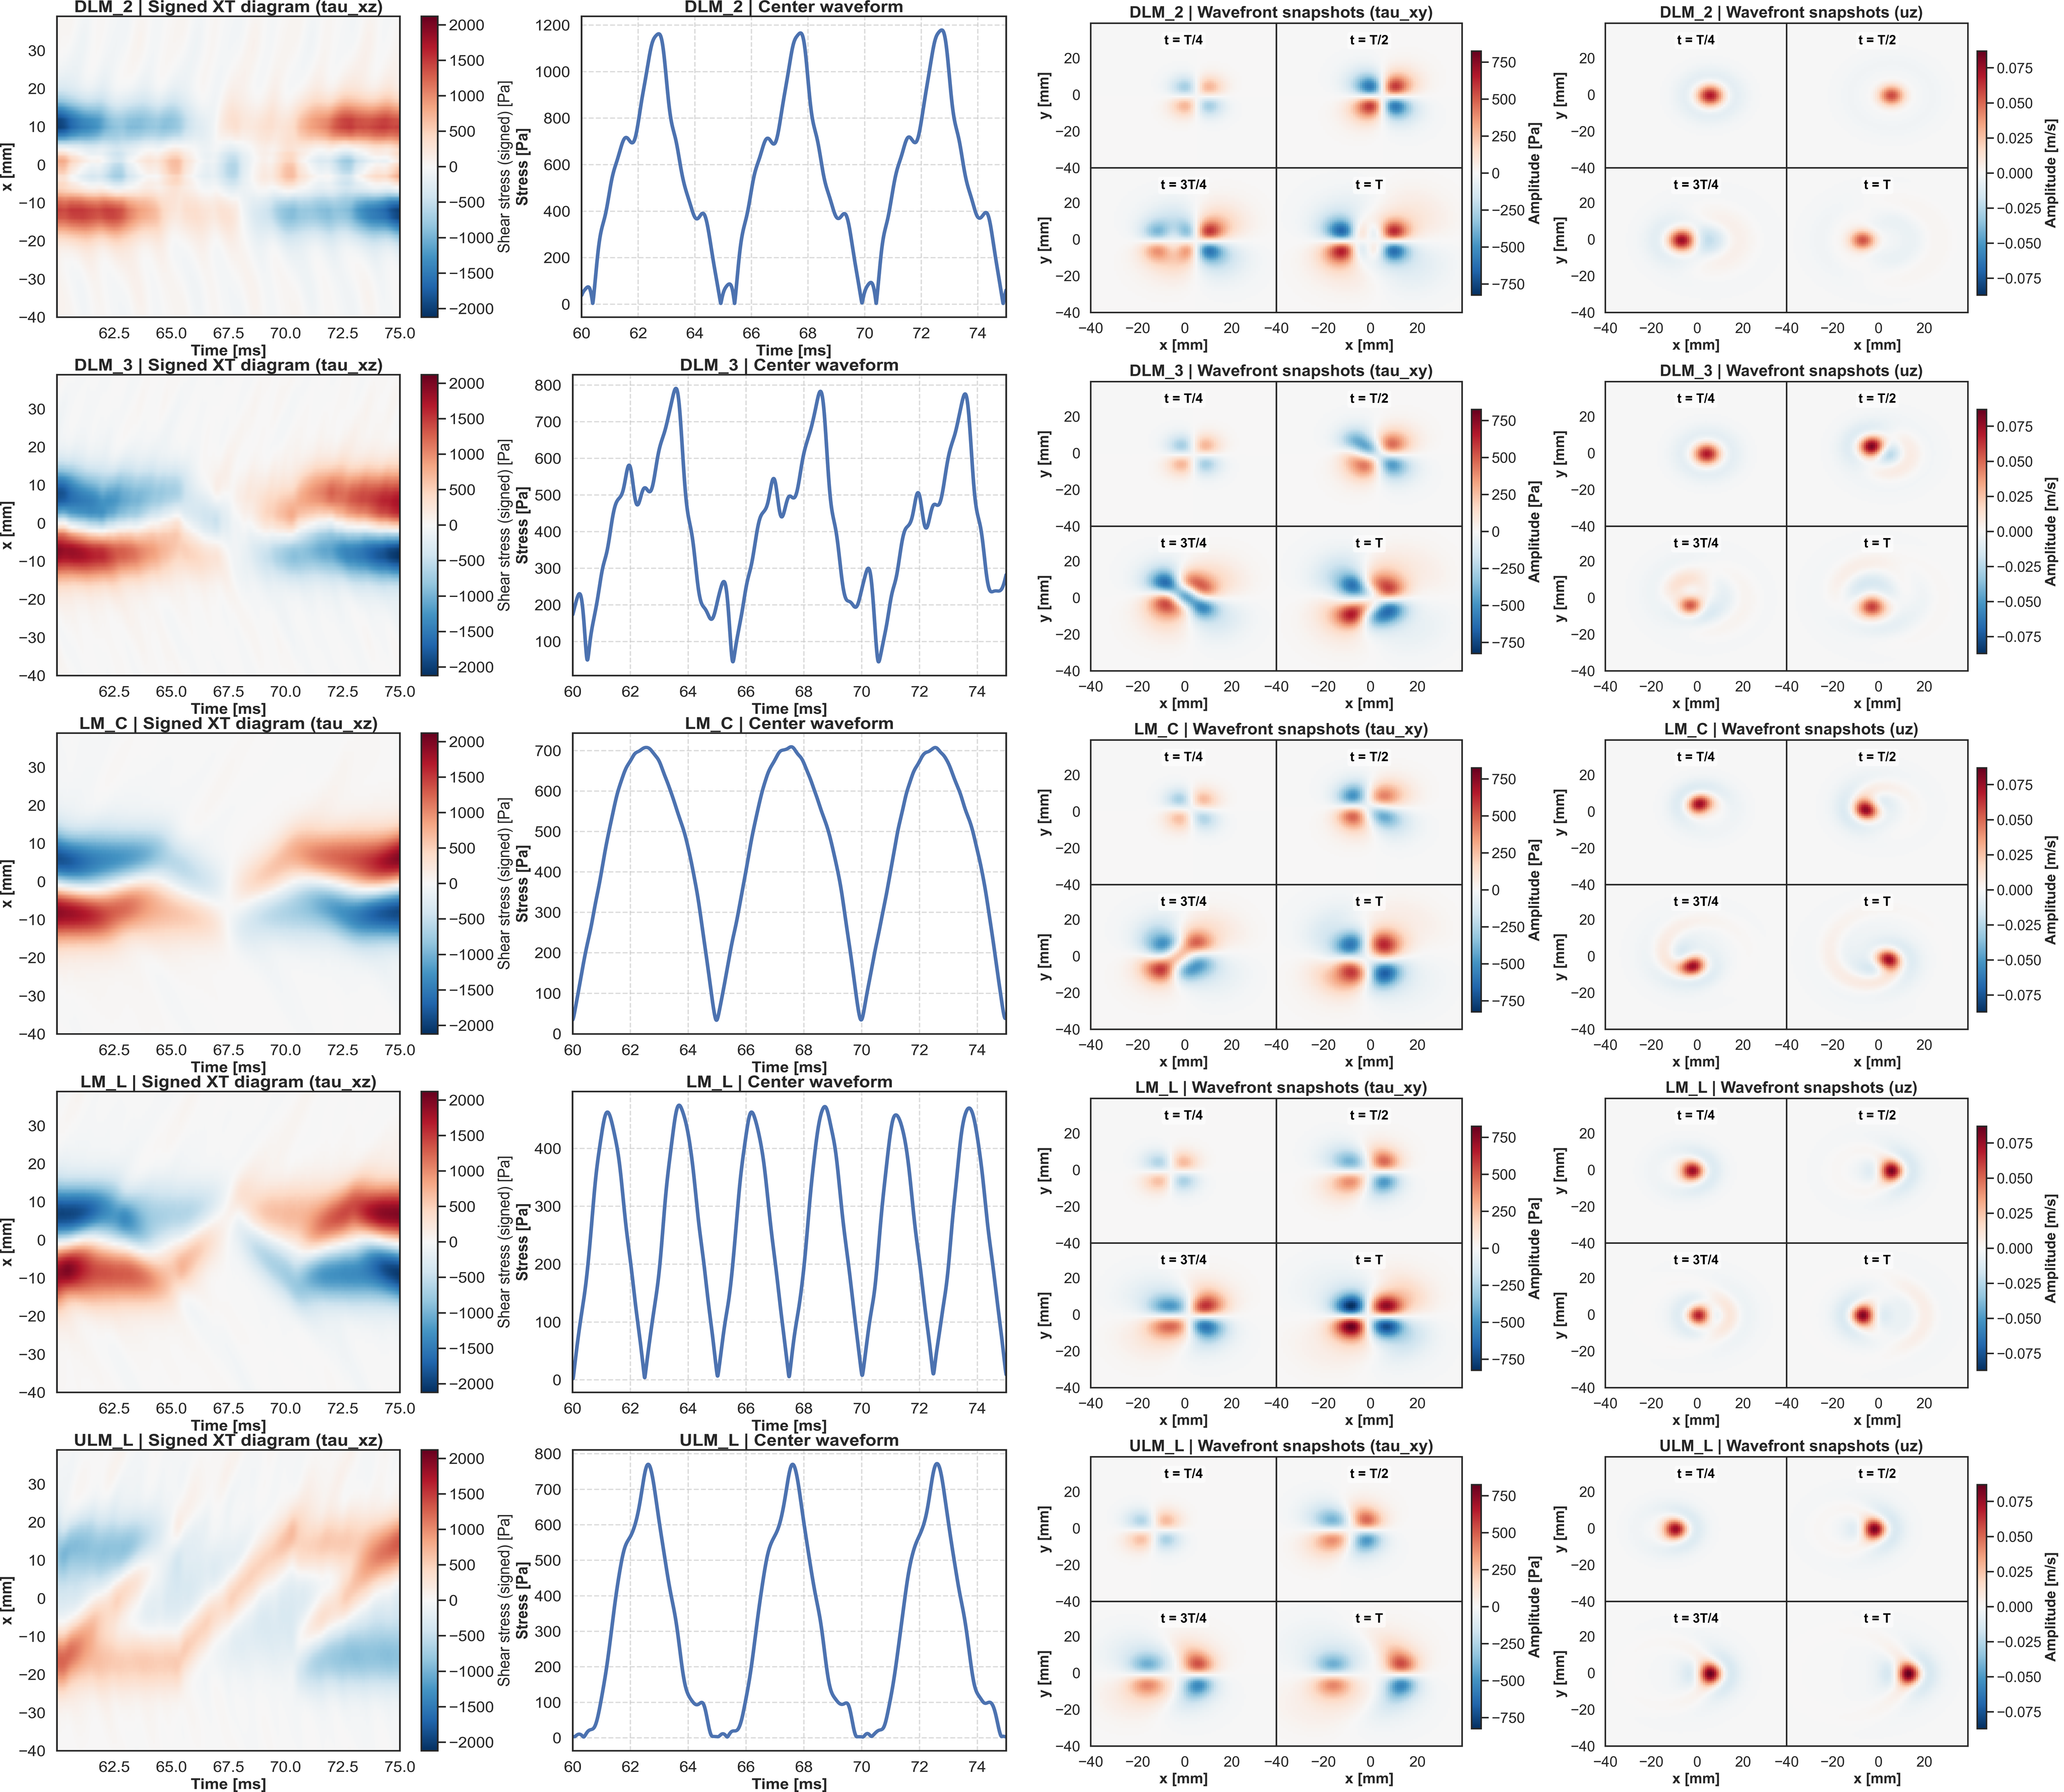
\includegraphics[width= \textwidth]{Figure_Sim_1_Full_Tempo.png}
    \caption{\textbf{Temporal evolution and wavefront dynamics.} The rows represent the modulation schemes: DLM-2, DLM-3, LM-C, LM-L, and ULM-L. The columns show: (1) \textbf{Signed XT Diagram ($\tau_{xz}$)}: Space-time plot of the shear stress component $\tau_{xz}$ along the x-axis, illustrating the wave propagation direction and interference patterns. (2) \textbf{Center Waveform}: Time history of the stress magnitude at the focal center, showing the temporal modulation envelope. (3) \textbf{Wavefront Snapshots ($\tau_{xy}$)}: Instantaneous spatial distributions of shear stress $\tau_{xy}$ at four phases ($t=T/4, T/2, 3T/4, T$) within a modulation cycle. (4) \textbf{Wavefront Snapshots ($u_z$)}: Corresponding snapshots of the vertical displacement velocity, highlighting the primary wave propagation.}
    \label{fig:supplementary_figure_sim_1_full_temporal}
\end{figure}

We normalized scalar maps by the global maximum:
\begin{equation}
    \tilde{M}^{(m)}(x,y)=\frac{M^{(m)}(x,y)}{\max_{m',x,y} M^{(m')}(x,y)},
\end{equation}

To ensure rigorous spectral analysis, we applied specific signal processing steps before computing frequency-domain metrics. For all temporal data extracted from the region of interest (ROI), we first removed the DC component (demeaning) to eliminate static stress bias:
\begin{equation}
    \tau_{\text{centered}}(t) = \tau(t) - \frac{1}{T}\int_0^T \tau(t) dt.
\end{equation}
Subsequently, we applied a Hanning window to the demeaned signal to suppress spectral leakage caused by the finite simulation duration, ensuring that the discrete Fourier transform (DFT) accurately reflected the dynamic energy distribution.

The simulations provide a mechanistic description of how \qty{200}{\hertz} modulation strategies generate different internal wave organizations. The numerical framework separates three determinants of tactile efficacy: surface trajectory, propagation delay, and tensorial stress redistribution.

To quantitatively capture the key physical mechanisms underlying these differences, we introduced two novel metrics: the Frequency Fidelity Index (FFI) and the Directional Wavefront Concentration Index (DWCI).

\textbf{Frequency Fidelity Index (FFI).} The FFI quantifies the proportion of shear wave energy that is faithfully maintained at the target modulation frequency (\qty{200}{\hertz}) versus being dispersed into higher harmonics. We computed the power spectrum $P(f)$ by summing the squared magnitude of the temporal Fast Fourier Transform (FFT) of the steady-state shear stress $\tau_{\text{roi\_steady}}(x,y,t)$ across the entire spatial ROI:
\begin{equation}
    P(f) = \sum_{x,y} \left| \mathcal{F}_t \{ \tau_{\text{roi\_steady}}(x,y,t) \} \right|^2.
\end{equation}
The FFI is then defined as the ratio of power at the fundamental frequency to the total power at the fundamental and its first three harmonics:
\begin{equation}
    \mathrm{FFI} = \frac{P(200)}{P(200)+P(400)+P(600)+P(800)}.
\end{equation}
A high FFI indicates that the modulation strategy effectively concentrates mechanical energy into the frequency band most sensitive to Pacinian corpuscles, avoiding wasteful frequency doubling.

\textbf{Directional Wavefront Concentration Index (DWCI).} The DWCI assesses the extent to which the shear wave field at \qty{200}{\hertz} is organized into a single, dominant directional propagation mode. For each shear stress component $c \in \{xy, xz, yz\}$, we extracted the complex field $A_c(x,y)$ at \qty{200}{\hertz} via temporal FFT. We then performed a 2D spatial Fourier transform to obtain the wavenumber spectrum:
\begin{equation}
    E_c(k_x, k_y) = \left|\mathcal{F}_{2D}\{A_c(x,y)\}\right|^2.
\end{equation}
Summing over components gives the total directional energy distribution $E_{\text{total}}(k_x, k_y) = \sum_c E_c(k_x, k_y)$. The DWCI is defined as the peak-to-total energy ratio in the wavenumber domain:
\begin{equation}
    \mathrm{DWCI} = \frac{\max(E_{\text{total}})}{\sum E_{\text{total}}}.
\end{equation}
This index penalizes scattered or multi-directional wave patterns (low DWCI) and rewards strategies like $ULM_L$ that generate a highly coherent, unidirectional wavefront (high DWCI).




\SupplementarySection{Computational neural dynamics modeling details}
\label{sec:computational_neural_dynamics_modeling_details}

We developed a minimal, mechanistically grounded peripheral neural model to test whether the psychophysical ranking of modulation strategies could be explained by cutaneous shear-wave propagation dynamics rather than static mechanical extrema.

The model specifically targets the Pacinian corpuscle (PC) / rapidly adapting type II (RAII) pathway. This choice is grounded in established psychophysical evidence showing that detection thresholds for vibrotactile stimuli above \qty{100}{\hertz} are determined almost exclusively by the PC system~\citep{johnsonRolesFunctionsCutaneous2001, handlerMechanosensoryNeuronsTouch2021}. While other mechanoreceptors (e.g., Meissner corpuscles) contribute to low-frequency flutter, the \qty{200}{\hertz} carrier envelope used here falls squarely within the PC's maximum sensitivity range. Furthermore, recent ultrastructural studies have highlighted the role of Lamellar Schwann Cells (LSCs) in tuning the dynamic sensitivity of the PC nerve terminal~\citep{ziolkowskiTouchSensationRequires2025}. Rather than explicitly modeling the complex biophysics of the LSC-neurite interaction, which would introduce unconstrained parameters, we abstract the inner core complex into an effective spatiotemporal integration kernel (Eq. 46). This formulation captures the functional role of the end-organ in summing coherent mechanical events while maintaining model parsimony.

We kept all model parameters fixed across conditions, allowing the modulation schemes to differ only through their input spatiotemporal mechanical fields.

The model inputs were the steady-state spatiotemporal shear-stress fields ($\tau_{xy}, \tau_{xz}, \tau_{yz}$) at \qty{1}{\milli\meter} depth. We used the steady-state window to focus on the sustained percept. A lattice of virtual receptors with uniform \qty{2}{\milli\meter} spacing covered the region of interest. For each receptor $i$ and shear component $c$, we removed the static bias:
\begin{equation}
    \tau^{\mathrm{dyn}}_{c}(r_j,t)=\tau_{c}(r_j,t)-\langle \tau_{c}(r_j,\cdot)\rangle_t,
\end{equation}
This reflects the Pacinian system's sensitivity to dynamic vibration~\citep{johanssonTactileSensoryCoding1983, johnsonRolesFunctionsCutaneous2001, handlerMechanosensoryNeuronsTouch2021}.

The model's central operation was a causal spatiotemporal integration step representing the summation of cutaneous surface waves. For receptor $i$ and shear component $c$:
\begin{equation}
    m_{c,i}(t)=\sum_{j \in \Omega_i} K(d_{ij})\,\tau^{\mathrm{dyn}}_{c}\!\left(r_j, t-\frac{d_{ij}}{c_s}\right),
\end{equation}
with
\begin{equation}
    d_{ij}=\lVert r_j-r_i \rVert,
    \qquad
    K(d_{ij})=\exp\!\left(-\frac{d_{ij}}{\lambda}\right).
\end{equation}
Here $c_s=\qty{5}{\meter\per\second}$ and $\lambda=\qty{4}{\milli\meter}$. This integral defines coherence: if a modulation strategy organizes the wavefront so that disturbances arrive with compatible timing, they add constructively.

We passed the delayed mechanical drive through a fixed band-pass filter representing the Pacinian channel:
\begin{equation}
    u_{c,i}(t)=(h_{\mathrm{PC}} * m_{c,i})(t),
\end{equation}
where $h_{\mathrm{PC}}$ is a fourth-order Butterworth band-pass filter (\qty{150}{\hertz}--\qty{300}{\hertz}). This penalized modulation schemes that shifted power into non-optimal harmonics.

A leaky integrate-and-fire element converted the filtered drive $u_{c,i}(t)$ into a spike train:
\begin{equation}
    \tau_m\frac{dV_{c,i}}{dt}=-V_{c,i}+g\,[u_{c,i}(t)]_{+},
\end{equation}
with $\tau_m=\qty{2}{\milli\second}$, $t_{\mathrm{ref}}=\qty{2}{\milli\second}$, $V_{\mathrm{th}}=1$, and $g=1$.

We quantified the steady-state response by combining firing rate and phase locking. Vector strength at \qty{200}{\hertz} was:
\begin{equation}
    VS_{c,i}=\left|\frac{1}{N_i}\sum_{k=1}^{N_i} \exp\!\left(\mathrm{i}2\pi f_0 t_k\right)\right|,
\end{equation}
We defined a component-specific effective coding weight:
\begin{equation}
    w_{c,i}=r_{c,i}\,VS_{c,i}.
\end{equation}
This metric assigns high weight only to receptors that fire strongly and remain temporally aligned with the modulation period.

A directional max-pooling rule combined the three shear channels:
\begin{equation}
    w_i=\max\left(w_{xy,i},w_{xz,i},w_{yz,i}\right).
\end{equation}
This retains sensitivity to the shear component that best expresses the local mechanically effective mode.

The population intensity score for modulation method $m$ was:
\begin{equation}
    S^{(m)}_{\mathrm{intensity}}=\log\!\left(1+\sum_i w_i\right).
\end{equation}

To compare with psychophysics, we standardized the scores:
\begin{equation}
    \hat{S}^{(m)}=\frac{S^{(m)}_{\mathrm{intensity}}-\mu_S}{\sigma_S},
\end{equation}
The predicted probability that method $A$ is preferred over $B$ is:
\begin{equation}
    P(A \succ B)=\frac{1}{1+\exp\left[-\left(\hat{S}^{(A)}-\hat{S}^{(B)}\right)\right]}.
\end{equation}

The model reproduced the principal behavioral ranking. The standardized neural intensity score was highest for $ULM_L$ ($z=1.196$), followed by $DLM_2$ ($z=0.634$), $DLM_3$ ($z=0.079$), $LM_C$ ($z=-0.135$), and $LM_L$ ($z=-1.773$). $ULM_L$ excels because unidirectional motion at the surface-wave speed favors constructive arrival and preserves the \qty{200}{\hertz} rhythm. $LM_L$ degrades coherence through direction reversal and frequency doubling.

\SupplementarySection{Sensitivity of Spatiotemporal Coherence to Scan Speed (Mach Number) in Unidirectional Lateral Modulation}
\label{sec:sensitivity_spatiotemporal_coherence_scan_speed}

This study hypothesizes that tactile perception in ultrasonic haptics depends on the spatiotemporal coherence of cutaneous shear waves, governed by a Mach cone effect when focal scan speed matches surface wave speed. To test this hypothesis and verify that the superiority of $ULM_L$ is not simply due to unidirectional motion, we conducted a parameter sweep experiment manipulating the focal Mach number.

We used the k-Wave elastodynamic simulation framework described above. Fixed parameters were $f_0 = \qty{200}{\hertz}$ and $c_s = \qty{5}{\meter\per\second}$. We varied the $ULM_L$ trajectory length $L$ to achieve scan speeds $v = L/T$. We define the focal Mach number as $M = v/c_s$. We evaluated $M = 0.2, 0.5, 1.0, 1.2$, and $2.0$. The $M=1.2$ condition matches the $ULM_L$ stimulus used in the main experiments.

\begin{figure}[htbp]
    \centering
    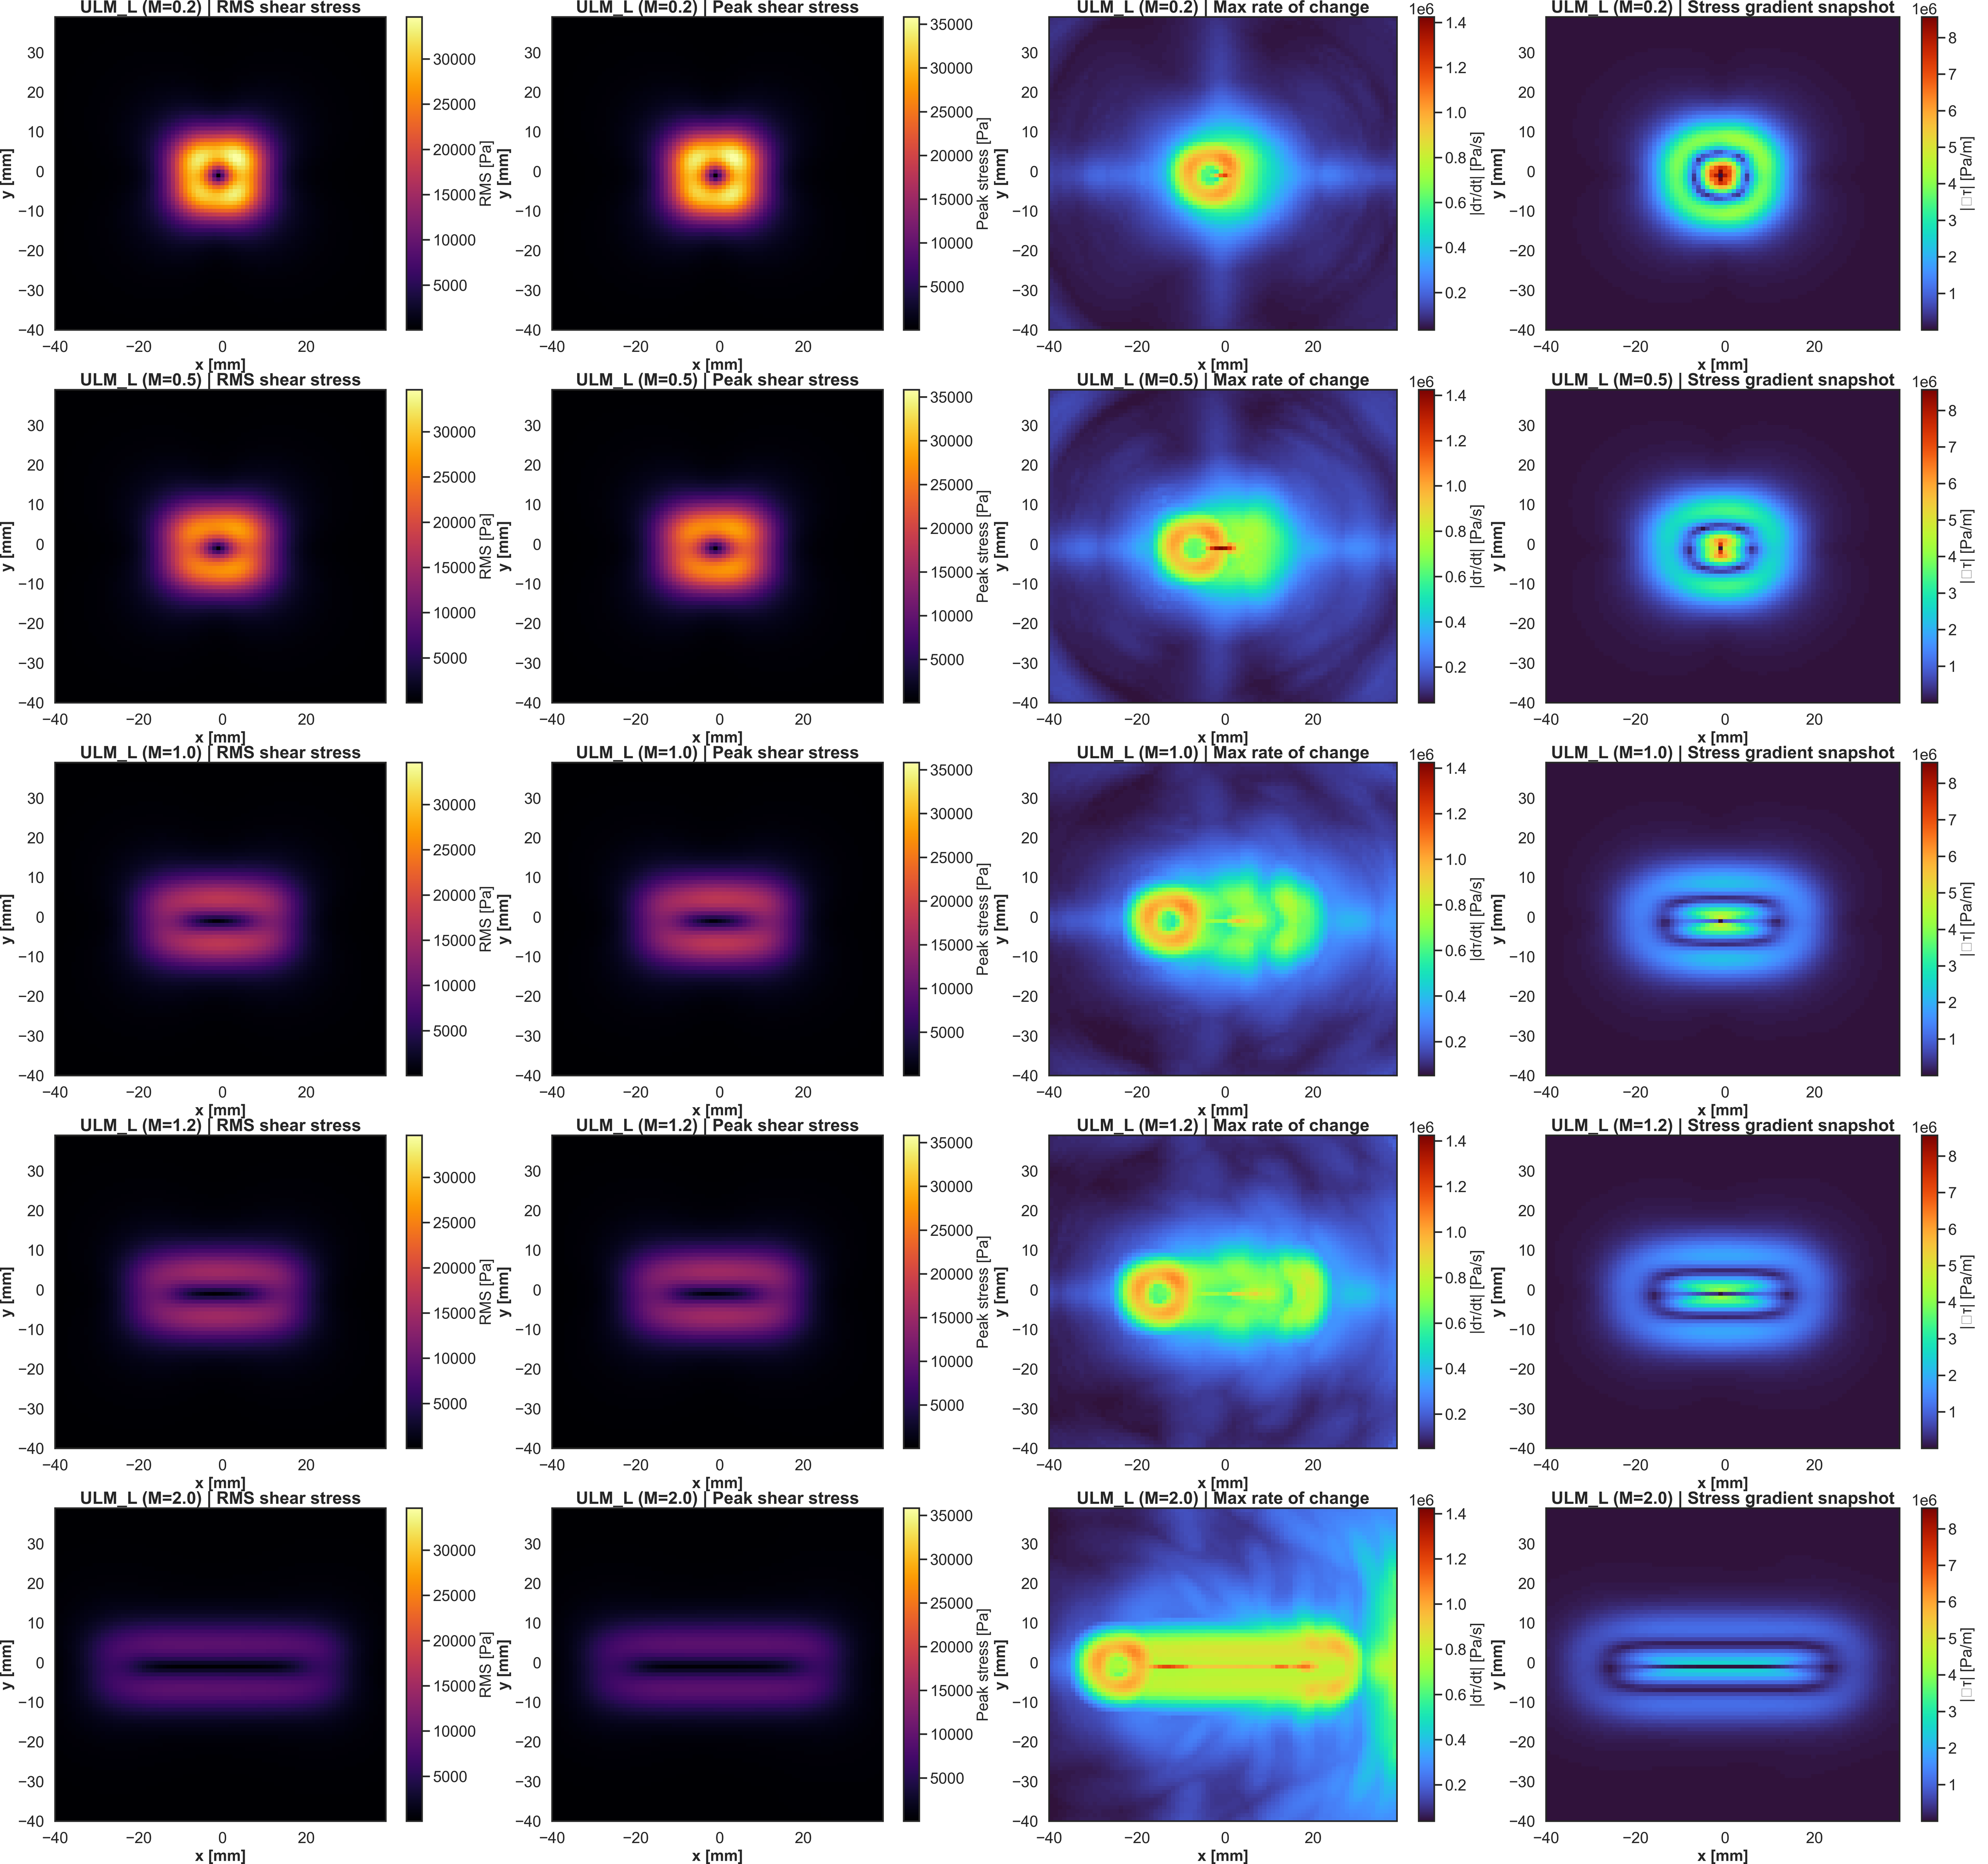
\includegraphics[width=\textwidth]{Figure_Supplementary_Sim_1_Full_Spatial.png}
    \caption{\textbf{Spatial distribution of stress metrics for unidirectional lateral modulation ($ULM_L$) at varying Mach numbers.} The rows correspond to different focal Mach numbers ($M = v/c_s$): 0.2, 0.5, 1.0, 1.2, and 2.0. The columns display, from left to right: (1) \textbf{RMS Shear Stress}, (2) \textbf{Peak Shear Stress}, (3) \textbf{Max Rate of Change} ($\max |d\boldsymbol{\tau}/dt|$), and (4) \textbf{Stress Gradient Snapshot} ($|\nabla \boldsymbol{\tau}|$). All metrics are evaluated at a depth of \qty{1}{\milli\meter}. Kinematic matching near $M \approx 1$ maximizes the dynamic impact (max rate of change) along the scan trajectory.}
    \label{fig:supplementary_figure_mach_sweep_spatial}
\end{figure}

\cref{fig:supplementary_figure_mach_sweep_spatial} presents the spatial distribution of stress metrics. In the subsonic regime ($M=0.2, 0.5$), acoustic energy concentrates within a small geometric center. Low-speed scanning generates the highest absolute local extremes (peak shear stress, max rate of change), but these are confined to a tiny area. As scan speed approaches shear wave speed ($M=1.0, 1.2$), local peak values decrease, but the high-stress distribution elongates along the scan axis, forming a coherent wake. Kinematic matching transforms a localized transient into a sustained, directional dynamic impact. In the supersonic regime ($M=2.0$), the focal point moves too rapidly, decoupling from the propagating waves. This disperses acoustic energy over a wide V-shaped wake, significantly reducing all physical metrics.

\begin{figure}[htbp]
    \centering
    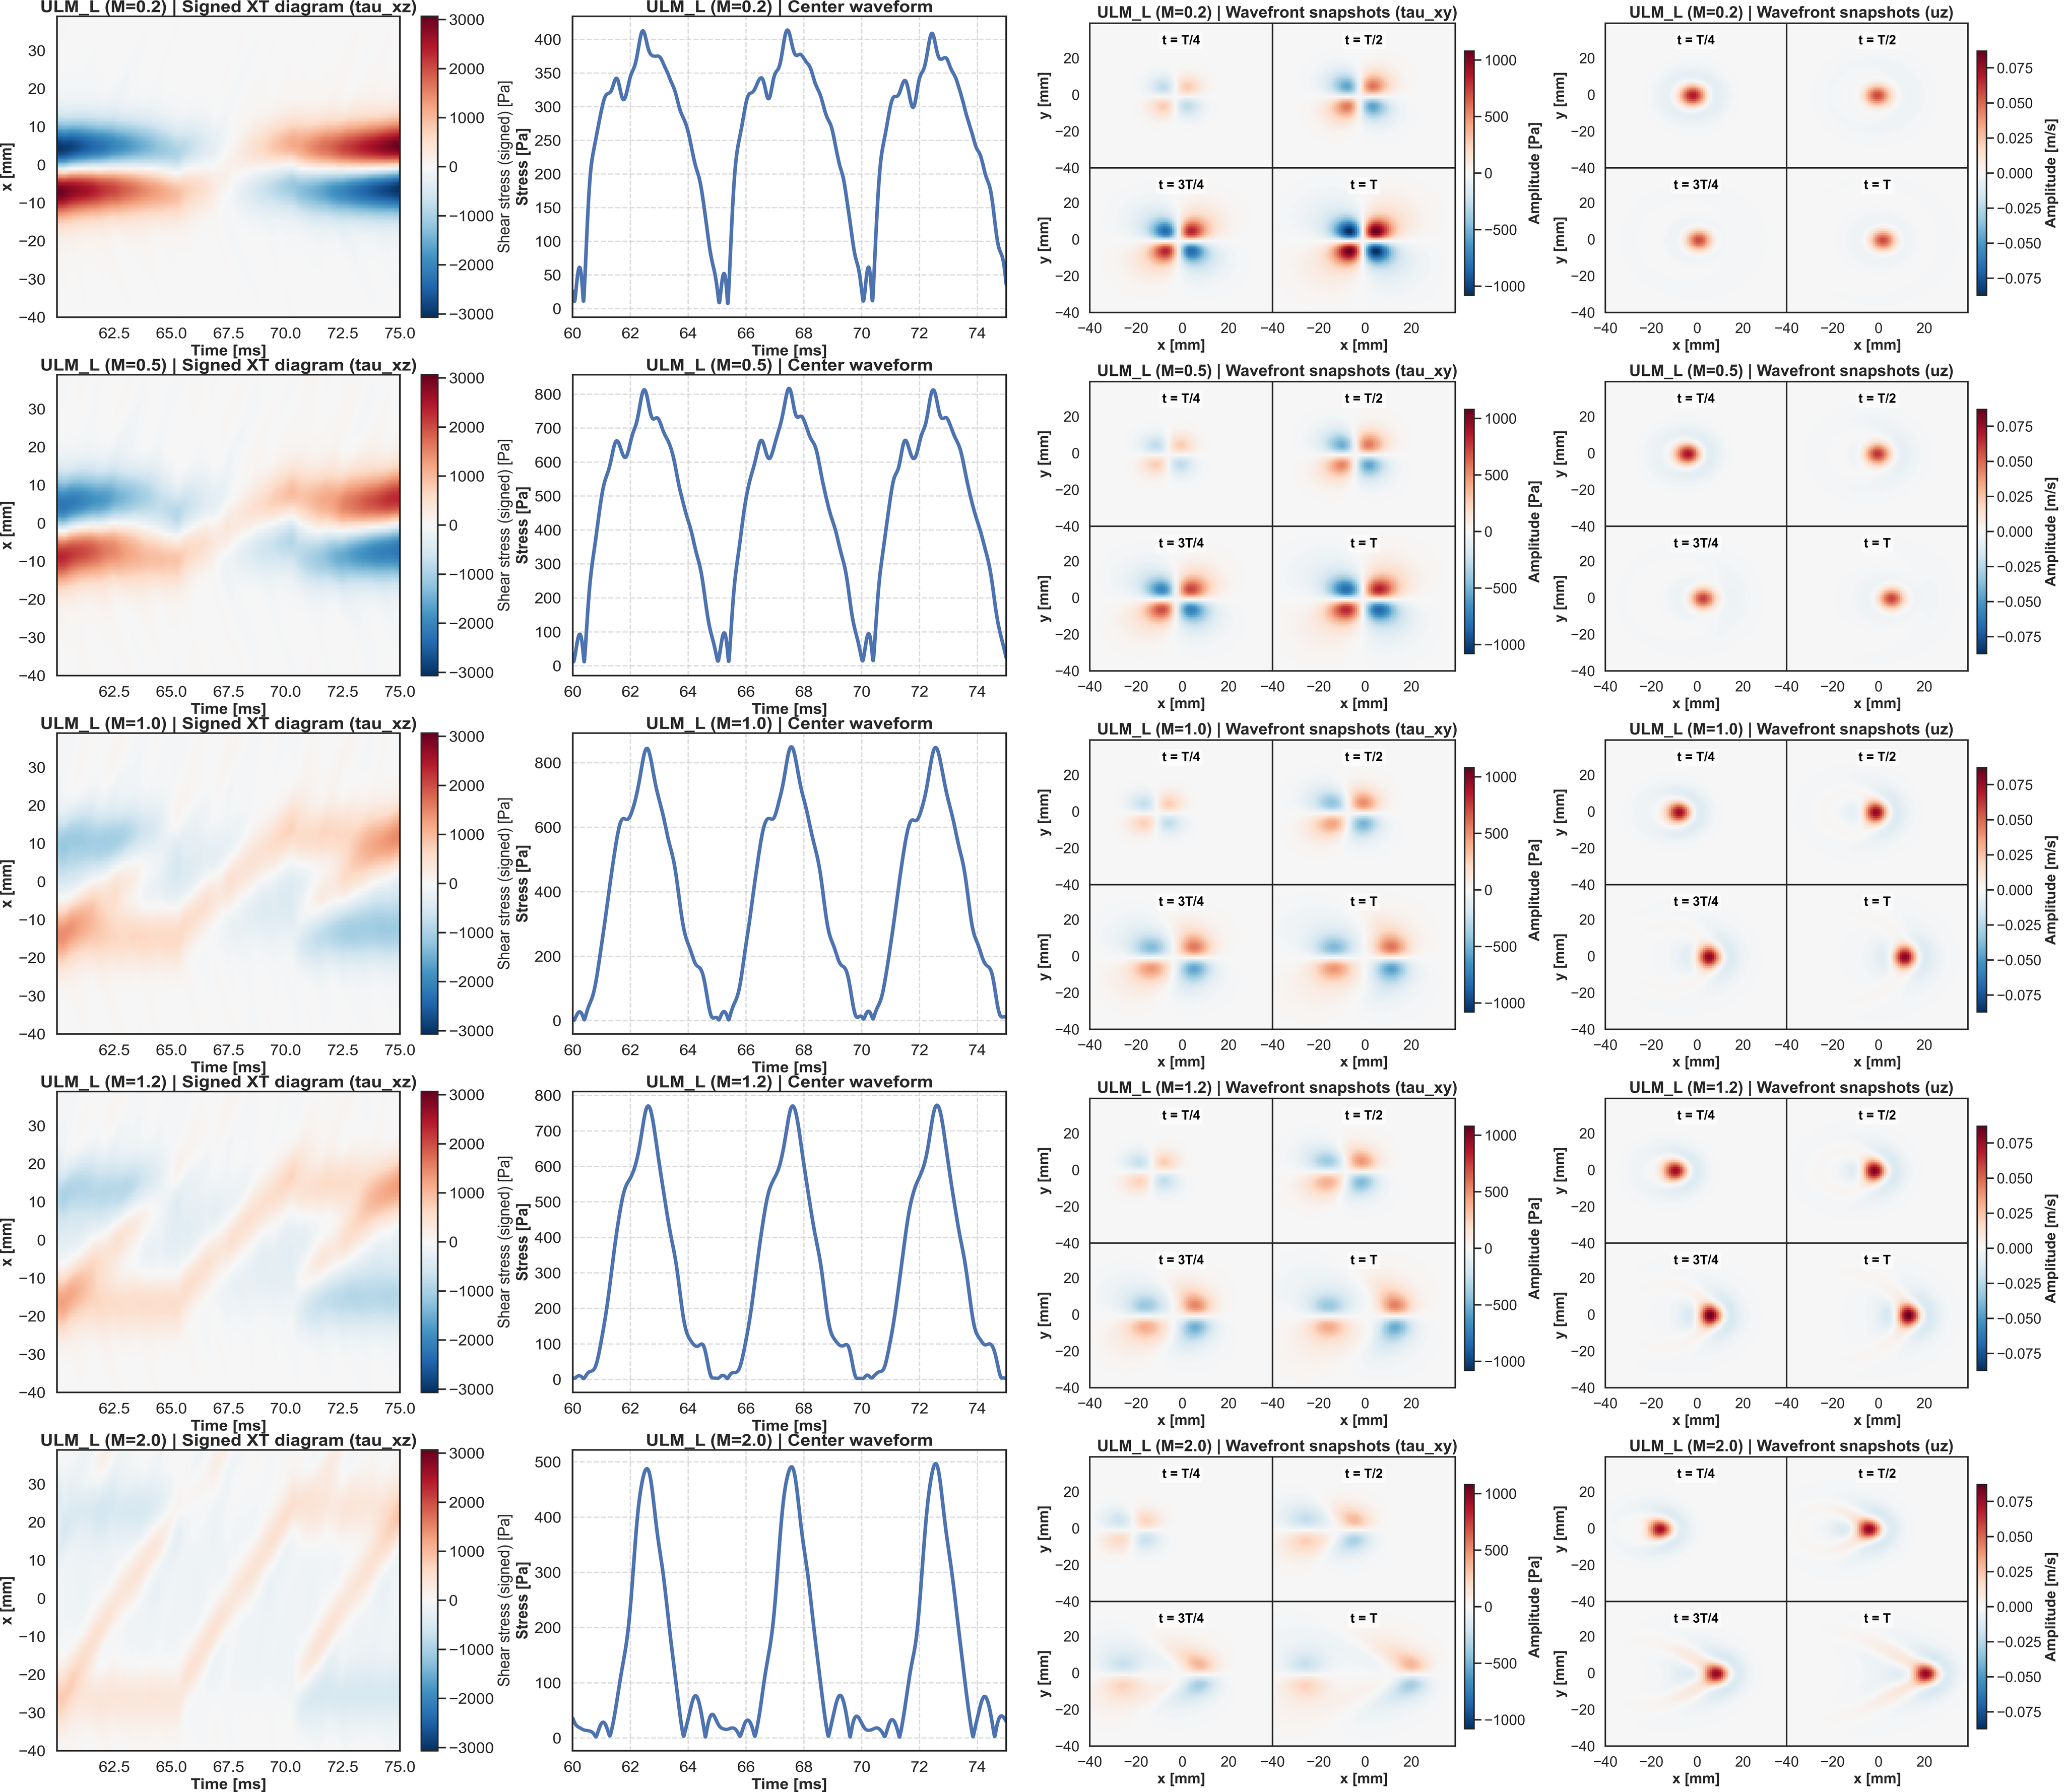
\includegraphics[width=\textwidth]{Figure_Supplementary_Sim_1_Full_Tempo.png}
    \caption{\textbf{Temporal evolution and wavefront dynamics for unidirectional lateral modulation ($ULM_L$) at varying Mach numbers.} The rows represent the focal Mach numbers: 0.2, 0.5, 1.0, 1.2, and 2.0. The columns show: (1) \textbf{Signed XT Diagram ($\tau_{xz}$)} along the scan axis, (2) \textbf{Center Waveform} showing the stress magnitude history at the focal center, (3) \textbf{Wavefront Snapshots ($\tau_{xy}$)} at four phases within a modulation cycle, and (4) \textbf{Wavefront Snapshots ($u_z$)} of the vertical displacement velocity. Transonic speeds ($M=1.0, 1.2$) demonstrate strong constructive interference, forming a coherent wave packet that travels with the focal point.}
    \label{fig:supplementary_figure_mach_sweep_temporal}
\end{figure}

Temporal evolution and wavefront dynamics (\cref{fig:supplementary_figure_mach_sweep_temporal}) elucidate the mechanism. Signed XT diagrams show that at subsonic speeds, the source moves slower than the emitted wavefronts, causing symmetrical outward radiation. At transonic speeds ($M=1.0, 1.2$), the source trajectory aligns with shear wave propagation. This allows newly generated stress to stack onto the forward-propagating wavefront. This coherent integration appears in the center waveform as a sharp compression peak and in wavefront snapshots as a concentrated leading edge. At supersonic speeds ($M=2.0$), the source outruns its shear waves, creating a wide trailing Mach cone and losing the sharp temporal compression.

To empirically validate these simulation findings and confirm that wave speed matching (the Mach cone effect) is the central mechanism for coherent integration and enhanced perception, we conducted a supplementary psychophysical paired-comparison experiment. We used the same 2-AFC paradigm and environmental controls as Experiment 1. The modulation frequency was fixed at \qty{200}{\hertz}, and we tested the five scan speeds for $ULM_L$ by varying the trajectory length: $M=0.2$ (highly subsonic, $L=\qty{5.0}{\milli\meter}$), $M=0.5$ (subsonic, $L=\qty{12.5}{\milli\meter}$), $M=1.0$ (exact wave speed match, $L=\qty{25}{\milli\meter}$), $M=1.2$ (near-match supersonic, $L=\qty{30}{\milli\meter}$), and $M=2.0$ (highly supersonic, $L=\qty{50}{\milli\meter}$).

A Bradley--Terry mixed-effects model revealed that the Mach matching regime dictates perceptual efficacy. In the intensity task, the exactly matched $M=1.0$ and near-matched $M=1.2$ conditions achieved the highest scores ($1.42$ and $1.40$, respectively), with no significant difference between them ($p=0.923$). The highly supersonic $M=2.0$ condition maintained a relatively high intensity score ($1.26$), not significantly lower than the matched conditions ($p>0.4$), indicating that once a Mach cone forms, it provides substantial wave compression. However, when the speed dropped to the subsonic regime ($M=0.5$ and $M=0.2$), where the Mach cone cannot form, perceived intensity collapsed dramatically (scores of $-0.76$ and $-3.32$, both significantly lower than all $M \ge 1.0$ conditions, $p<0.001$).

For spatial clarity, the $M=1.0$ condition provided the highest score ($0.47$), again not significantly different from $M=1.2$ ($0.36$, $p=0.505$). Crucially, while the highly supersonic $M=2.0$ condition retained high intensity, its spatial clarity score plummeted to $-0.14$, significantly lower than both matched conditions ($p<0.001$ against $M=1.0$, $p=0.003$ against $M=1.2$). This behavioral drop aligns perfectly with the physical wave dispersion and overly acute Mach cone angle observed in the $M=2.0$ simulations. In addition, reaction time data (Z-Log-RT) showed that participants made extremely rapid decisions when rejecting the highly subsonic $M=0.2$ condition against others, reflecting its unequivocally weak percept. Conversely, comparisons between the high-performing $M=1.0$ and $M=1.2$ conditions yielded the longest reaction times, indicating perceptual equivalence in the optimal wave-speed matching zone.

In conclusion, both the elastodynamic simulations and the psychophysical validation support our central hypothesis: the perceptual efficacy of spatiotemporal modulation fundamentally depends on the kinematic matching between focal scan speed and tissue shear wave speed. The superiority of $ULM_L$ derives from its ability to harness the Mach cone effect for coherent integration ($M \ge 1$), ensuring a directional, sustained mechanical drive. Furthermore, optimizing for both maximal perceptual intensity and sharp spatial localization requires tuning the scan speed closely to the wave speed ($M \approx 1.0 \sim 1.2$), avoiding both subsonic collapse and extreme supersonic dispersion.

\bibliography{SWIM}% common bib file

\end{document}
